%!TEX root=../../main.tex
\begin{chapterpage}{Multiple linear regression}
  \chaptertitle{Multiple linear regression}
  \label{multipleLinearRegression}
  \chaptersection{introductionMultipleLinearRegression}
  \chaptersection{simpleVsMultipleRegression}
  \chaptersection{evaluatingFitMultipleRegression}
  \chaptersection{generalMultipleRegression}
  \chaptersection{categoricalMoreThanTwoLevels}
  \chaptersection{reanalyzingStatinDataSet}
  \chaptersection{interactionRegression}
  \chaptersection{modelSelection}
  \chaptersection{ANOVAandRegression}
  \chaptersection{multLinRegrNotes}
\end{chapterpage}
\renewcommand{\chapterfolder}{ch_multiple_linear_regression_oi_biostat}

\index{multiple linear regression|textbf}

\chapterintro{{\large In most practical settings, more than one explanatory variable is likely to be associated with a response. This chapter discusses how the ideas behind simple linear regression can be extended to a model with multiple predictor variables. 

There are several applications of multiple regression. One of the most common applications in a clinical setting is estimating an association between a response variable and primary predictor of interest while adjusting for possible confounding variables. Sections~\ref{introductionMultipleLinearRegression} and \ref{simpleVsMultipleRegression} introduce the multiple regression model by examining the possible association between cognitive function and the use of statins after adjusting for potential confounders. Section~\ref{modelSelection} discusses another application of multiple regression\textemdash constructing a model that effectively explains the observed variation in the response variable. 

The other sections in the chapter outline general principles of multiple regression, including the statistical model, methods for assessing quality of model fit, categorical predictors with more than two levels, interaction, and the connection between ANOVA and regression.  The methods used to conduct hypothesis tests and construct confidence intervals for regression coefficients extend naturally from simple to multiple linear regression, so the section on the statistical model for multiple regression can be treated as optional.}}


\section{Introduction to multiple linear regression}
\label{introductionMultipleLinearRegression}

Statins are a class of drugs widely used to lower cholesterol. There are two main types of cholesterol: low density lipoprotein (LDL) and high density lipoprotein (HDL).\footnote{Total cholesterol level is the sum of LDL and HDL levels.} Research suggests that adults with elevated LDL may be at risk for adverse cardiovascular events such as a heart attack or stroke. In 2013, a panel of experts commissioned by the American College of Cardiology and the American Heart Association recommended that statin therapy be considered in individuals who either have any form of atherosclerotic cardiovascular disease\footnote{i.e., arteries thickening and hardening with plaque} or have LDL cholesterol levels $\geq 190$ mg/dL, individuals with Type II diabetes ages 40 to 75 with LDL between 70 to 189 mg/dL, and non-diabetic individuals ages of 40 to 75 with a predicted probability of future clogged arteries of at least 0.075.\footnote{Stone NJ, et al. 2013 ACC/AHA Guideline on the Treatment of Blood Cholesterol to Reduce Atherosclerotic Cardiovascular Risk in Adults Circulation. 2014;129:S1-S45. DOI: 10.1161/01.cir.0000437738.63853.7a}


\index{data!PREVEND|(}

Health policy analysts have estimated that if the new guidelines were to be 
followed, almost half of Americans ages 40 to 75 and nearly all men over 60 would be prescribed a statin. However, some physicians have raised the question of whether treatment with a statin might be associated with an increased risk of cognitive decline.\footnote{Muldoon, Matthew F., et al. Randomized trial of the effects of simvastatin on cognitive functioning in hypercholesterolemic adults. The American journal of medicine 117.11 (2004): 823-829.}\textsuperscript{,}\footnote{King, Deborah S., et al. Cognitive impairment associated with atorvastatin and simvastatin. Pharmacotherapy: The Journal of Human Pharmacology and Drug Therapy 23.12 (2003): 1663-1667.} Older adults are at increased risk for cardiovascular disease, but also for cognitive decline. A study by Joosten, et al. examined the association of statin use and other variables with cognitive ability in an observational cohort of 4,095 participants from the Netherlands who were part of the larger PREVEND study introduced in Section~\ref{examiningScatterPlots}.\footnote{Joosten H, Visser ST, van Eersel ME, Gansevoort RT, Bilo HJG, et al. (2014) Statin Use and Cognitive Function: Population-Based Observational Study with Long-Term Follow- Up. PLoS ONE 9(12): e115755. doi:10.1371/ journal.pone.0115755} The analyses presented in this chapter are based on a random sample of 500 participants from the cohort.\footnote{The random sample are accessible as \data{prevend.samp} in the \data{oibiostat} \textsf{R} package.}

The investigators behind the Joosten study anticipated an issue in the analysis\textemdash statins are used more often in older adults than younger adults, and older adults suffer a natural cognitive decline. Age is a potential \term{confounder} in this setting. If age is not accounted for in the analysis, it may seem that cognitive decline is more common among individuals prescribed statins, simply because those prescribed statins are simply older and more likely to have reduced cognitive ability than those not prescribed statins.

\textD{\newpage}

\begin{figure}[t]
	\centering
	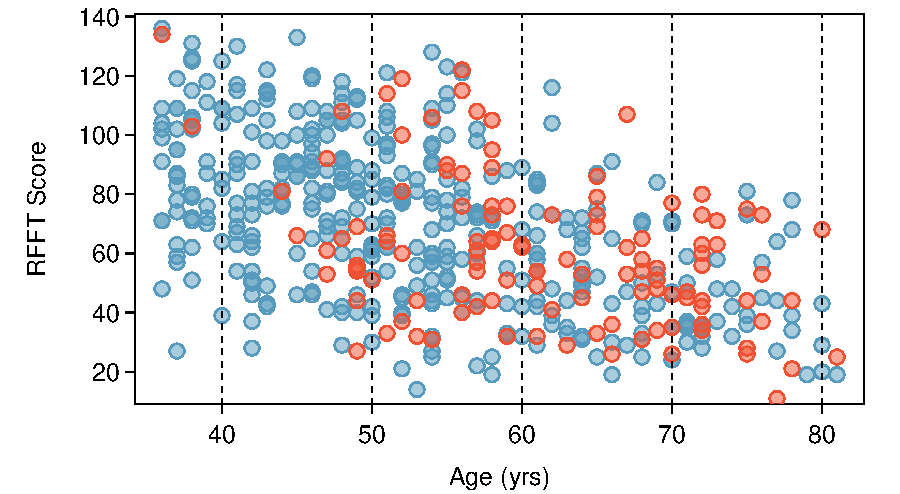
\includegraphics[width=0.85\textwidth]
	{ch_multiple_linear_regression_oi_biostat/figures/prevendAgeRFFTConfounderPlot/prevendAgeRFFTConfounderPlot}
	\caption{A scatterplot showing \var{age} vs. \var{RFFT} in \data{prevend.samp}. Statin users are represented with red points; participants not using statins are shown as blue points.}
	\label{prevendAgeRFFTConfounderPlot}
\end{figure}

Figure~\ref{prevendAgeRFFTConfounderPlot} visually demonstrates why age is a potential confounder for the association between statin use and cognitive function, where cognitive function is measured via the Ruff Figural Fluency Test (RFFT). Scores range from 0 (worst) to 175 (best). The blue points indicate individuals not using statins, while red points indicate statin users. First, it is clear that age and statin use are associated, with statin use becoming more common as age increases; the red points are more prevalent on the right side of the plot. Second, it is also clear that age is associated with lower RFFT scores; ignoring the colors, the point cloud drifts down and to the right. However, a close inspection of the plot suggests that for ages in relatively small ranges (e.g., ages 50-60), statin use may not be strongly associated with RFFT score\textemdash there are approximately as many red dots with low RFFT scores as with high RFFT scores in a given age range. In other words, for subsets of participants with approximately similar ages, statin use may not be associated with RFFT. Multiple regression provides a way to estimate the association of statin use with RFFT while adjusting for age; i.e., accounting for the underlying relationship between age and statin use.


\section{Simple versus multiple regression}
\label{simpleVsMultipleRegression}

A simple linear regression model can be fit for an initial examination of the association between statin use and RFFT score,
\[
E(\text{RFFT}) = \beta_0 + \beta_{\text{Statin}}(\text{Statin}).
\label{RFFTStatinModel}
\]

RFFT scores in \data{prevend.samp} are approximately normally distributed, ranging between approximately 10 and 140, with no obvious outliers (Figure~\ref{prevendRFFTHist}). The least squares regression line shown in Figure~\ref{prevendStatinRFFTDotPlot} has a negative slope, which suggests a possible negative association. 

\begin{figure}[ht]
	\centering
	\subfigure[]{
		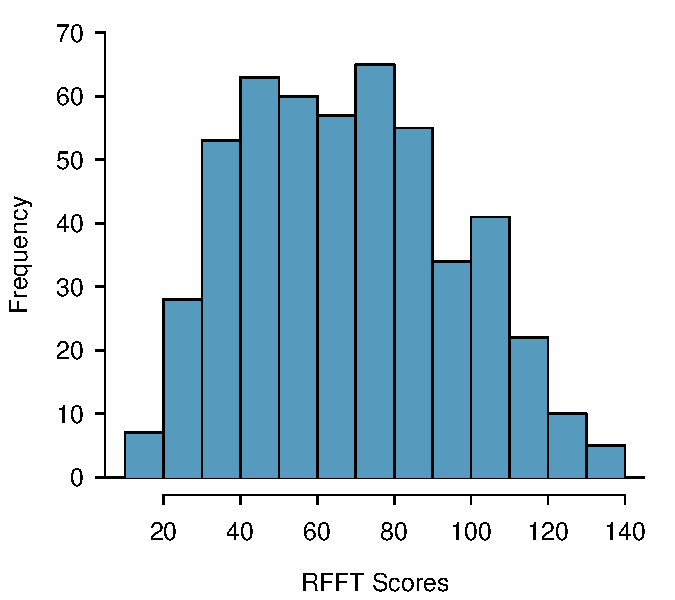
\includegraphics[width=0.485\textwidth]
		{ch_multiple_linear_regression_oi_biostat/figures/prevendStatinRFFTPlots/prevendRFFTHist}
		\label{prevendRFFTHist}
	}
	\subfigure[]{
		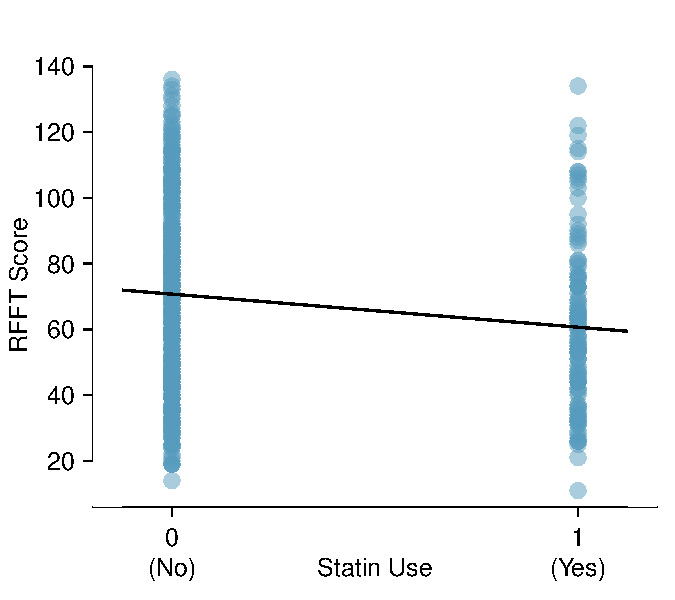
\includegraphics[width=0.485\textwidth]
		{ch_multiple_linear_regression_oi_biostat/figures/prevendStatinRFFTPlots/prevendStatinRFFTDotPlot}
		\label{prevendStatinRFFTDotPlot}
	}
	\caption{\subref{prevendRFFTHist} Histogram of RFFT scores. \subref{prevendStatinRFFTDotPlot} Scatterplot of RFFT score versus statin use in \data{prevend.samp}. The variable \var{Statin} is coded \resp{1} for statin users, and \resp{0} otherwise.}
	\label{prevendStatinRFFTPlot}
\end{figure}

Figure~\ref{prevendRFFTStatinRegression} gives the parameter estimates of the least squares line, and indicates that the association between RFFT score and statin use is highly significant. On average, statin users score approximately 10 points lower on the RFFT. However, even though the association is statistically significant, it is potentially misleading since the model does not account for the underlying relationship between age and statin use. The association between age and statin use visible from Figure~\ref{prevendAgeRFFTConfounderPlot} is even more apparent in Figure~\ref{prevendStatinAgeBoxPlot}, which shows that the median age of statin users is about 10 years higher than the median age of individuals not using statins. 

% latex table generated in R 3.3.2 by xtable 1.8-2 package
% Fri Jan  5 10:49:51 2018
\begin{figure}[ht]
\centering
\begin{tabular}{rrrrr}
  \hline
 & Estimate & Std. Error & t value & Pr($>$$|$t$|$) \\ 
  \hline
(Intercept) & 70.7143 & 1.3808 & 51.21 & 0.0000 \\ 
  Statin & -10.0534 & 2.8792 & -3.49 & 0.0005 \\ 
   \hline
\end{tabular}
\caption{\textsf{R} summary output for the simple regression model of RFFT versus statin use in \data{prevend.samp}.} 
\label{prevendRFFTStatinRegression}
\end{figure}

 \begin{figure}[h]
 	\centering
 	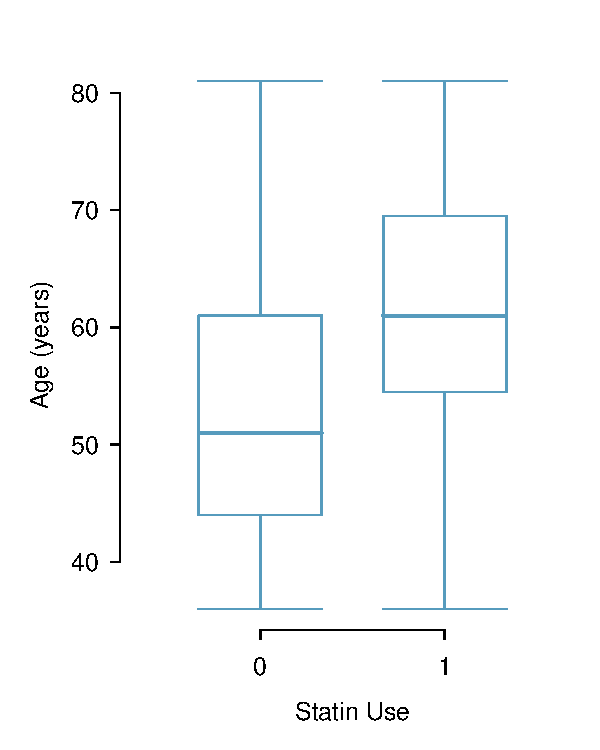
\includegraphics[width=0.5\textwidth]
 	{ch_multiple_linear_regression_oi_biostat/figures/prevendStatinAgeBoxPlot/prevendStatinAgeBoxPlot.pdf}
 	\caption{Boxplot of age by statin use in \data{prevend.samp}. The variable \var{Statin} is coded \resp{1} for statin users, and \resp{0} otherwise.}
 	\label{prevendStatinAgeBoxPlot}
 \end{figure}

\textD{\newpage}

Multiple regression allows for a model that incorporates both statin use and age,
 \[
    E(\text{RFFT}) = \beta_0 + \beta_{\text{Statin}}(\text{Statin}) + \beta_{\text{Age}}(\text{Age}).
	\label{RFFTStatinAgeEquation}
 \]
In statistical terms, the association between \var{RFFT} and \var{Statin} is being estimated after adjusting for \var{Age}. This is an example of one of the more important applications of multiple regression: estimating an association between a response variable and primary predictor of interest while adjusting for possible confounders. In this setting, statin use is the primary predictor of interest.

The principles and assumptions behind the multiple regression model are introduced more formally in Section~\ref{generalMultipleRegression}, along with the method used to estimate the coefficients. Figure~\ref{prevendRFFTStatinAgeRegression} shows the parameter estimates for the model from \textsf{R}. 
% latex table generated in R 3.3.2 by xtable 1.8-2 package
% Fri Jan  5 11:04:43 2018
\begin{figure}[ht]
\centering
\begin{tabular}{rrrrr}
  \hline
 & Estimate & Std. Error & t value & Pr($>$$|$t$|$) \\ 
  \hline
(Intercept) & 137.8822 & 5.1221 & 26.92 & 0.0000 \\ 
  Statin & 0.8509 & 2.5957 & 0.33 & 0.7432 \\ 
  Age & -1.2710 & 0.0943 & -13.48 & 0.0000 \\ 
   \hline
\end{tabular}
\caption{\textsf{R} summary output for the multiple regression model of RFFT versus statin use and age in \data{prevend.samp}.} 
\label{prevendRFFTStatinAgeRegression}
\end{figure}
 
\begin{examplewrap}
\begin{nexample}{Using the parameter estimates in Figure~\ref{prevendRFFTStatinAgeRegression}, write the prediction equation for the linear model. How does the predicted RFFT score for a 67-year-old not using statins compare to that of an individual of the same age who does use statins?}\label{prevendRFFTStatinAgeExample}%
The equation of the linear model is
\[\widehat{\text{RFFT}} = 137.8822 + 0.8509(\text{Statin}) - 1.2710(\text{Age}). \]	

The predicted RFFT score for a 67-year-old not using statins (\texttt{Statin = 0}) is
\[\widehat{\text{RFFT}} = 137.8822 + \textcolor{blue}{(0.8509)(0)} - (1.2710)(67) = 52.7252. \]

The predicted RFFT score for a 67-year-old using statins (\texttt{Statin = 1}) is
\[\widehat{\text{RFFT}} = 137.8822 + \textcolor{blue}{(0.8509)(1)} - (1.2710)(67) = 53.5761. \]

The two calculations differ only by the value of the coefficient $\beta_{\text{Statin}}$, 0.8509.\footnotemark{} Thus, for two individuals who are the same age, the model predicts that RFFT score will be 0.8509 higher in the individual taking statins; statin use is associated with a small increase in RFFT score.
\end{nexample}
\end{examplewrap}
\footnotetext{In most cases, predictions do not need to be calculated to so many significant digits, since the coefficients are only estimates. This example uses the additional precision to illustrate the role of the coefficients.}

\index{multiple linear regression!prediction}

\begin{examplewrap}
\begin{nexample}{Suppose two individuals are both taking statins; one individual is 50 years of age, while the other is 60 years of age. Compare their predicted RFFT scores.} 

From the model equation, the coefficient of age $\beta_{\text{Age}}$ is -1.2710; an increase in one unit of age (i.e., one year) is associated with a decrease in RFFT score of -1.2710, when statin use is the same. Thus, the individual who is 60 years of age is predicted to have an RFFT score that is about 13 points lower ($(-1.2710)(10) = -12.710$) than the individual who is 50 years of age. 

This can be confirmed numerically:

The predicted RFFT score for a 50-year-old using statins is
\[\widehat{\text{RFFT}} = 137.8822 + (0.8509)(1) - (1.2710)(50) = 75.1831. \]

The predicted RFFT score for a 60-year-old using statins is
\[\widehat{\text{RFFT}} = 137.8822 + (0.8509)(1) - (1.2710)(60) = 62.4731. \]

The scores differ by $62.4731 - 75.1831 = - 12.710.$
\end{nexample}
\end{examplewrap}

\textD{\newpage}

\begin{exercisewrap}
\begin{nexercise}
What does the intercept represent in this model? Does the intercept have interpretive value?\footnotemark{}
\end{nexercise}
\end{exercisewrap}
\footnotetext{The intercept represents an individual with value \resp{0} for both \var{Statin} and \var{Age}; i.e., an individual not using statins with age of 0 years. It is not reasonable to predict RFFT score for a newborn, or to assess statin use; the intercept is meaningless and has no interpretive value.}

As in simple linear regression, $t$-statistics can be used to test hypotheses about the slope coefficients; for this model, the two null hypotheses are $H_0: \beta_{\text{Statin}} = 0$ and $H_0: \beta_{\text{Age}} = 0$. The $p$-values for the tests indicate that at significance level $\alpha = 0.05$, the association between RFFT score and statin use is not statistically significant, but the association between RFFT score and age is significant. 

In a clinical setting, the interpretive focus lies on reporting the nature of the association between the primary predictor and the response and specifying which confounders have been adjusted for. The results of the analysis might be summarized as follows\textemdash
\begin{quotation}
	Although the use of statins appeared to be associated with lower RFFT scores when no adjustment was made for possible confounders, statin use is not significantly associated with RFFT score in a regression model that adjusts for age. 
\end{quotation}

The results shown in Figure~\ref{prevendRFFTStatinAgeRegression} do not provide information about either the quality of the model fit or its value as a prediction model. The next section describes the residual plots that can be used to check model assumptions and the use of $R^2$ to estimate how much of the variability in the response variable is explained by the model.

There is an important aspect of these data that should not be overlooked. The data do not come from a study in which participants were followed as they aged; i.e., a longitudinal study. Instead, this study was a cross-sectional study, in which patient age, statin use, and RFFT score were recorded for all participants during a short time interval. While the results of the study support the conclusion that older patients tend to have lower RFFT scores, they cannot be used to conclude that scores decline with age in individuals; there were no repeated measurements of RFFT taken as individual participants aged. Older patients come from an earlier birth cohort, and it is possible, for instance, that younger participants have more post-secondary school education or better health practices generally; such a cohort effect may have some explanatory effect on the observed association. The details of how a study is designed and how data are collected should always be taken into account when interpreting study results. 

\index{data!PREVEND|)}


\section{Evaluating the fit of a multiple regression model}
\label{evaluatingFitMultipleRegression}

\subsection{Using residuals to check model assumptions}
\label{modelCheckMultipleRegression}

\index{residuals!regression}
\index{multiple linear regression!residuals}
\index{multiple linear regression!assumptions}

The assumptions behind multiple regression are essentially the same as the four assumptions listed in Section~\ref{examiningScatterPlots} for simple linear regression. The assumption of linearity is extended to multiple regression by assuming that when only one predictor variable changes, it is linearly related to the change in the response variable.  Assumption 2 becomes the slightly more general assumption that the residuals have approximately constant variance. Assumptions 3 and 4 do not change; it is assumed that the observations on each case are independent and the residuals are approximately normally distributed.

Since it is not possible to make a scatterplot of a response variable against several simultaneous predictors, residual plots become even more essential as tools for checking modeling assumptions. 

\index{multiple linear regression!residual plots}
To assess the linearity assumption, examine plots of residuals against each of the predictors. These plots might show an nonlinear trend that could be corrected with a transformation. The scatterplot of residual values versus age in Figure~\ref{prevendStatinAgeResidPlot} shows no apparent nonlinear trends. It is not necessary to assess linearity against a categorical predictor, since a line drawn through two points (i.e., the means of the two groups) is necessarily linear.

\begin{figure}[h]
	\centering
	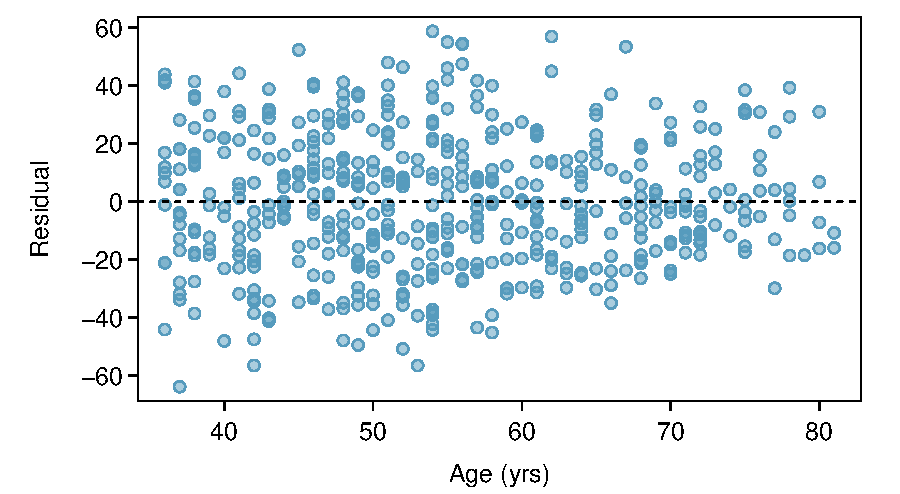
\includegraphics[width=0.8\textwidth]
	{ch_multiple_linear_regression_oi_biostat/figures/prevendStatinAgeResidPlot/prevendStatinAgeResidPlot.pdf}
	\caption{Residuals versus age in the model for RFFT vs statins and age in the PREVEND data.}
	\label{prevendStatinAgeResidPlot}
\end{figure}

\textD{\newpage}

Since each case has one predicted value and one residual, regardless of the number of predictors, residuals can still be plotted against predicted values to assess the constant variance assumption. The scatterplot in the left panel of Figure~\ref{prevendStatinAgeResidNormPlot} shows that the variance of the residuals is slightly smaller for lower predicted values of RFFT, but is otherwise approximately constant.

\index{normal probability plot}

Just as in simple regression, normal probability plots can be used to check the normality assumption of the residuals. The normal probability plot in the right panel of Figure~\ref{prevendStatinAgeResidNormPlot} shows that the residuals from the model are reasonably normally distributed, with only slight departures from normality in the tails.

\begin{figure}[h]
	\centering
	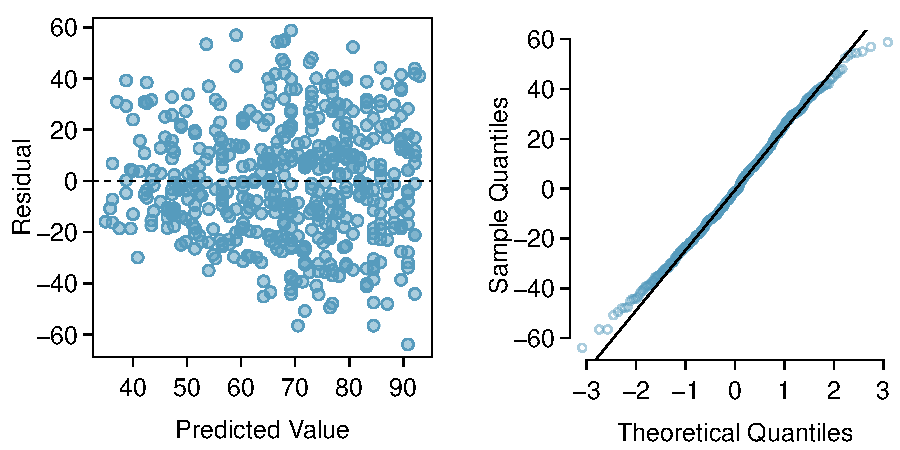
\includegraphics[width=0.8\textwidth]
	{ch_multiple_linear_regression_oi_biostat/figures/prevendStatinAgeResidNormPlot/prevendStatinAgeResidNormPlot.pdf}
	\caption{Residual plots from the linear model for RFFT versus statin use and age in \data{prevend.samp}.}
	\label{prevendStatinAgeResidNormPlot}
\end{figure}

\index{data!developmental disability support|(}

\begin{examplewrap}
\begin{nexample}{Section~\ref{exploratoryDataAnalysis} featured a case study examining the evidence for ethnic discrimination in the amount of financial support offered by the State of California to individuals with developmental disabilities. Although an initial look at the data suggested an association between \var{expenditures} and \var{ethnicity}, further analysis suggested that age is a confounding variable for the relationship.\vspace{3mm}

A multiple regression model can be fit to these data to model the association between \var{expenditures}, \var{age}, and \var{ethnicity} in a subset that only includes data from Hispanics and White non-Hispanics. Two residual plots from the model fit for 
\[E(\text{expenditures}) = \beta_0 +  \beta_{\text{ethnicity}}(\text{ethnicity}) + \beta_{\text{age}}(\text{age}) \]
are shown in Figure~\ref{ddsAgeEthnicityResidNormPlot}. From these plots, assess whether a linear regression model is appropriate for these data.}

The model assumptions are clearly violated. The residual versus fitted plot	shows obvious patterns; the residuals do not scatter randomly about the $y = 0$ line. Additionally, the variance of the residuals is not constant around the $y = 0$ line. As shown in the normal probability plot, the residuals show marked departures from normality, particularly in the upper tail; although this skewing may be partially resolved with a log transformation, the patterns in the residual versus fitted plot are more problematic.

Recall that a residual is the difference between an observed value and expected value; for an observation $i$, the residual equals $y_i - \hat{y}_i$. Positive residuals occur when a model's predictions are larger than the observed value, and vice versa for negative residuals. In the residual versus fitted plot, it can be seen that in the middle range of predicted values, the model consistently under-predicts expenditures; on the upper and lower ends, the model over-predicts. This is a particularly serious issue with the model fit. 

A single linear regression model is not appropriate for these data. For a more detailed examination of the model residuals, refer to Chapter 7, Lab 2. With some subsetting according to age cohort, it can be reasonable to use linear regression for modeling these data.
\end{nexample}
\end{examplewrap}

\begin{figure}[h]
	\centering
	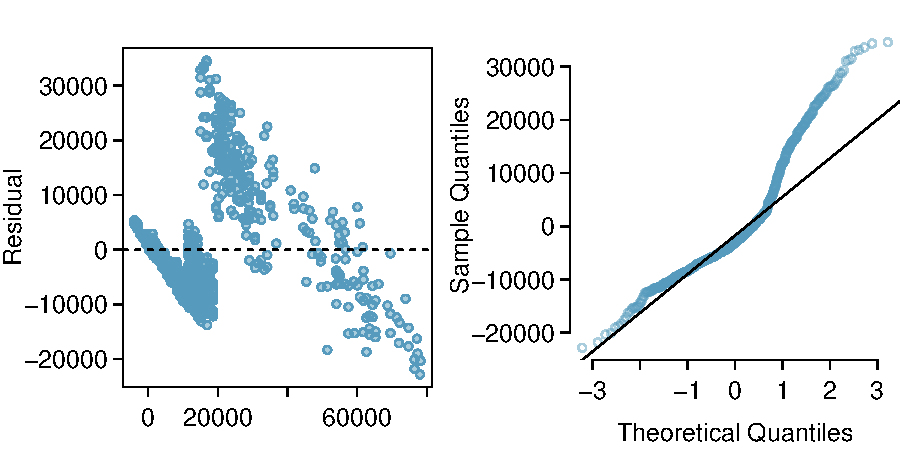
\includegraphics[width=0.8\textwidth]
	{ch_multiple_linear_regression_oi_biostat/figures/ddsAgeEthnicityResidNormPlot/ddsAgeEthnicityResidNormPlot.pdf}
	\caption{Residual versus fitted values plot and residual normal probability plot from the linear model for expenditures versus ethnicity and age for a subset of \data{dds.discr}.}
	\label{ddsAgeEthnicityResidNormPlot}
\end{figure}

\index{data!developmental disability support|)}


\textD{\newpage}


\subsection{Using $R^2$ and adjusted $R^2$ with multiple regression}
\index{adjusted r squared@adjusted $R^2$ ($R_{adj}^2$)|(}

Section~\ref{RSquaredLinearRegression} provided two definitions of the $R^2$ statistic\textemdash it is the square of the correlation coefficient $r$ between a response and the single predictor in simple linear regression, and equivalently, it is the proportion of the variation in the response variable explained by the model.  In statistical terms, the second definition can be written as 
\[
   R^2 = \frac{\text{Var}(y_i) - \text{Var}(e_i)}
   {\text{Var}(y_i)} = 1 - \frac{\text{Var}(e_i)}{\text{Var}(y_i)},
   \label{RSquareDefinition}\]
where $y_i$ and $e_i$ denote the response and residual values for the
$i^{\text{th}}$ case.

The first definition cannot be used in multiple regression, since there is a correlation coefficient between each predictor and the response variable. However, since there is a single set of residuals, the second definition remains applicable. 

Although $R^2$ can be calculated directly from the equation, it is rarely calculated by hand since statistical software includes $R^2$ as a standard part of the summary output for a regression model.\footnote{In \textsf{R} and other software, $R^2$ is typically labeled 'multiple R-squared'.} In the model with response \var{RFFT} and predictors \var{Statin} and \var{Age}, $R^2 = 0.2852$.  The model explains almost 29\% of the variability in RFFT scores, a considerable improvement over the model with \var{Statin} alone ($R^2 = 0.0239$).

Adding a variable to a regression model always increases the value of $R^2$. Sometimes that increase is large and clearly important, such as when age is added to the model for RFFT scores. In other cases, the increase is small, and may not be worth the added complexity of including another variable. The \term{adjusted R-squared} is often used to balance predictive ability with complexity in a multiple regression model. Like $R^2$, the adjusted $R^2$ is routinely provided in software output. 

\begin{onebox}{Adjusted $\mathbf{R^2}$ as a tool for model assessment}
The \termsub{adjusted $\mathbf{R^2}$}{adjusted r squared@adjusted $R^2$ ($R_{adj}^2$)} is computed as
\begin{align*}
R_{adj}^{2} = 1-\frac{\text{Var}(e_i) / (n-p-1)}{\text{Var}(y_i) / (n-1)}
	= 1-\frac{\text{Var}(e_i)}{\text{Var}(y_i)} \times
    \frac{n-1}{n-p-1},
\end{align*}
where $n$ is the number of cases used to fit the model and $p$ is the number of predictor variables in the model.
\end{onebox}

Essentially, the adjusted $R^2$ imposes a penalty for including additional predictors that do not contribute much towards explaining the observed variation in the response variable. The value of the adjusted $R^2$ in the model with both \var{Statin} and \var{Age} is 0.2823, which is essentially the same as the $R^2$ value of 0.2852. The additional predictor \var{Age} considerably increases the strength of the model, resulting in only a small penalty to the $R^2$ value.

While the adjusted $R^2$ is useful as a statistic for comparing models, it does not have an inherent interpretation like $R^2$. Students often confuse the interpretation of $R^2$ and adjusted $R^2$; while the two are similar, adjusted $R^2$ is \emph{not} the proportion of variation in the response variable explained by the model. The use of adjusted $R^2$ for model selection will be discussed in Section~\ref{modelSelection}.


\section{The general multiple linear regression model}
\label{generalMultipleRegression}
 
This section provides a compact summary of the multiple regression model and contains more mathematical detail than most other sections; the next section, Section~\ref{categoricalMoreThanTwoLevels}, discusses categorical predictors with more than two levels. The ideas outlined in this section and the next are illustrated with an extended analysis of the PREVEND data in Section~\ref{reanalyzingStatinDataSet}. 
 
\subsection{Model parameters and least squares estimation}
\index{multiple linear regression!general model}

For multiple regression, the data consist of a response variable $Y$ and $p$ explanatory variables $X_1, X_2,\ldots, X_p$.   Instead of the simple regression model 
 $${Y} = \beta_{0} + \beta_{1}X + {\varepsilon},$$
 multiple regression has the form
 $${Y} = \beta_{0} +
     \beta_{1}X_{1} + \beta_{2}X_{2} + \beta_{3}X_{3} + \dots +
     \beta_{p}X_{p} + \varepsilon,$$
or equivalently
 $$E(Y) = \beta_{0} + 
     \beta_{1}X_{1} + \beta_{2}X_{2} + \beta_{3}X_{3} + \dots +
     \beta_{p}X_{p},
	 \label{multipleRegressionModel}
	 $$ 
since the normally distributed error term $\varepsilon$ is assumed to have mean 0. Each predictor $x_i$ has an associated coefficient $\beta_i$.  In simple regression, the slope coefficient $\beta$ captures the change in the response variable $Y$ associated with a one unit change in the predictor $X$.  In multiple regression, the coefficient $\beta_j$ of a predictor $X_j$ denotes the change in the response variable $Y$ associated with a one unit change in $X_j$ when none of the other predictors change; i.e., each $\beta$ coefficient in multiple regression plays the role of a slope, as long as the other predictors are not changing.

Multiple regression can be thought of as the model for the mean of the response $Y$ in a population where the mean depends on the values of the predictors, rather than being constant. For example, consider a setting with two binary predictors such as statin use and sex; the predictors partition the population into four subgroups, and the four predicted values from the model are estimates of the mean in each of the four groups.

\textD{\newpage}

\begin{exercisewrap}
\begin{nexercise}
Figure~\ref{prevendRFFTStatinGenderRegression} shows an estimated regression model for \var{RFFT} with predictors \var{Statin} and \var{Gender}, where \var{Gender} is coded 0 for males and 1 for females.\footnotemark{} Based on the model, what are the estimated mean RFFT scores for the four groups defined by these two categorical predictors?\footnotemark{}
\end{nexercise}
\end{exercisewrap}
\addtocounter{footnote}{-1}
\footnotetext{Until recently, it was common practice to use gender to denote biological sex. Gender is different than biological sex, but this text uses the original names in published datasets.}
\addtocounter{footnote}{1}
\footnotetext{The prediction equation for the model is $\widehat{\text{RFFT}} = 70.41 - 9.97(\text{Statin}) + 0.61(\text{Gender})$. Both \texttt{Statin} and \texttt{Gender} can take on values of either \resp{0} or \resp{1}; the four possible subgroups are statin non-user / male (\texttt{0}, \texttt{0}), statin non-user / female (\texttt{0}, \texttt{1}), statin user / male (\texttt{1}, \texttt{0}), statin user / female (\texttt{1}, \texttt{1}). Predicted RFFT scores for these groups are 70.41, 71.02, 60.44, and 61.05, respectively.}

% latex table generated in R 3.3.2 by xtable 1.8-2 package
% Fri Jan  5 11:21:50 2018
\begin{figure}[ht]
\centering
\begin{tabular}{rrrrr}
  \hline
 & Estimate & Std. Error & t value & Pr($>$$|$t$|$) \\ 
  \hline
(Intercept) & 70.4068 & 1.8477 & 38.11 & 0.0000 \\ 
  Statin & -9.9700 & 2.9011 & -3.44 & 0.0006 \\ 
  Gender & 0.6133 & 2.4461 & 0.25 & 0.8021 \\ 
   \hline
\end{tabular}
\caption{\textsf{R} summary output for the multiple regression model of RFFT versus statin use and sex in \data{prevend.samp}.}
\label{prevendRFFTStatinGenderRegression}
\end{figure}

Datasets for multiple regression have $n$ cases, usually indexed algebraically by $i$, where $i$ takes on values from 1 to $n$; 1 denotes the first case in the dataset and $n$ denotes the last case.  The dataset \data{prevend.samp} contains $n = 500$ observations.  Algebraic representations of the data must indicate both the case number and the predictor in the set of $p$ predictors. For case $i$ in the dataset, the variable $X_{ij}$ denotes predictor $X_j$; the response for case $i$ is simply $Y_i$, since there can only be one response variable. The dataset \data{prevend.samp} has many possible predictors, some of which are examined later in this chapter.  The analysis in Section~\ref{simpleVsMultipleRegression} used $p=2$ predictors, \var{Statin} and \var{Age}.

Just as in Chapter~\ref{probability}, upper case letters are used when thinking of data as a set of random observations subject to sampling from a population, and lower case letters are used for observed values. In a dataset, it is common for each row to contain the information on a single case; the observations in row $i$ of a dataset with $p$ predictors can be written as $(y_i, x_{i1}, x_{i2}, \ldots, x_{ip})$.

For any given set of estimates $b_1, b_2,\ldots,b_p$ and predictors $x_{i1},x_{i2},\ldots,x_{ip}$, predicted values of the response can be calculated using
\[
   \hat{y}_i = b_0 + b_1 x_{i1} + b_2 x_{i2} +\cdots + b_p x_{ip},
\]
where $b_0, b_1, \dots, b_p$ are estimates of the coefficients $\beta_0, \beta_1, \dots, \beta_p$ obtained using the principle of least squares estimation. 

\index{multiple linear regression!residuals}
As in simple regression, each prediction has an associated residual, which is the difference between the observed value $y_i$ and the predicted value $\hat{y_i}$, or $e_i = y_i - \hat{y}_i$. The least squares estimate of the model is the set of estimated coefficients $b_0, b_1, \ldots b_p$ that minimizes $e_1^2 + e_2^2 + \cdots e_n^2$. Explicit formulas for the estimates involve advanced matrix theory, but are rarely used in practice.  Instead, estimates are calculated using software such as as \textsf{R}, Stata, or Minitab.


\textD{\newpage}


\subsection{Hypothesis tests and confidence intervals}

\index{multiple linear regression!hypothesis tests}
\index{multiple linear regression!confidence intervals}

\subsubsection{Using $t$-tests for individual coefficients}

The test of the null hypothesis $H_0: \beta_k = 0$ is a test of whether the predictor $X_k$ is associated with the response variable. When a coefficient of a predictor equals 0, the predicted value of the response does not change when the predictor changes; i.e., a value of 0 indicates there is no association between the predictor and response. Due to the inherent variability in observed data, an estimated coefficient $b_k$ will almost never be 0 even when the model coefficient $\beta_k$ is. Hypothesis testing can be used to assess whether the estimated coefficient is significantly different from 0 by examining the ratio of the estimated coefficient to its standard error.

When the assumptions of multiple regression hold, at least approximately, this ratio has a $t$-distribution with $n - (p + 1) =n - p - 1$ degrees of freedom when the model coefficient is 0. The formula for the degrees of freedom follows a general rule that appears throughout statistics\textemdash the degrees of freedom for an estimated model is the number of cases in the dataset minus the number of estimated parameters.  There are $p + 1$ parameters in the multiple regression model, one for each of the $p$ predictors and one for the intercept.

\index{sampling distribution!regression coefficient}

\begin{onebox}{Sampling distributions of estimated coefficients}
Suppose 
\[
\hat{y} = b_0 + b_1 x_{i} + b_2 x_{i} +\cdots + b_p x_{i}
\]
is an estimated multiple regression model from a dataset with $n$ observations on the response and predictor variables, and let $b_k$ be one of the estimated coefficients.  Under the hypothesis $H_0: \beta_k = 0$, the standardized statistic
\[
      \frac{b_k}{\textrm{s.e.}(b_k)}
\]
has a $t$-distribution with $n - p - 1$ degrees of freedom.
\end{onebox}

This sampling distribution can be used to conduct hypothesis tests and construct confidence intervals.

\begin{onebox}{Testing a hypothesis about a regression coefficient}
A test of the two-sided hypothesis
\[
  H_0: \beta_k = 0 \text{ vs. } H_A: \beta_k \ne 0
\]
is rejected with significance level $\alpha$ when 
\[
     \frac{|b_k|}{\textrm{s.e.}(b_k)} > t_{\text{df}}^\star,
\]
where $t_{\text{df}}^\star$ is the point on a $t$-distribution with $n - p - 1$ degrees of freedom and area $(1 - \alpha/2)$ in the left tail.
\end{onebox}

\textD{\newpage}

For one-sided tests, $t_{\text{df}}^\star$ is the point on a $t$-distribution with $n - p - 1$ degrees of freedom and area $(1 - \alpha)$ in the left tail. A one-sided test of $H_0$ against $H_A: \beta_k > 0$ rejects when the standardized coefficient is greater than  $ t_{\text{df}}^\star$; a one-sided test of $H_0$ against $H_A: \beta_k < 0$  rejects when the standardized coefficient is less than $-t_{\text{df}}^\star$. 

\begin{onebox}{Confidence intervals for regression coefficient}
A two-sided $100(1 - \alpha)$\% confidence interval for the model coefficient $\beta_k$ is 
\[
     b_k \pm {\textrm{s.e.}(b_k)} \times t_{\text{df}}^\star.
\]
\end{onebox}

All statistical software packages provide an estimate $s$ of the standard deviation of the residuals $\epsilon$.


\subsubsection{The $F$-statistic for an overall test of the model}
\index{multiple linear regression!$F$-statistic}

When all the model coefficients are 0, the predictors in the model, considered as a group, are not associated with the response; i.e., the response variable is not associated with any linear combination of the predictors. The $F$-statistic is used to test this null hypothesis of no association, using the following idea.  

The variability of the predicted values about the overall mean response can be estimated by
\[
   \text{MSM} =  \frac{\sum_i(\hat{y}_i - \overline{y})^2}{p}.
\]
In this expression, $p$ is the number of predictors and is the degrees of freedom of the numerator sum of squares (derivation not given here).  The term \termsub{MSM}{model sum of squares (MSM)} is called the model sum of squares because it reflects the variability of the values predicted by the model ($\hat{y_i}$) about the mean ($\overline{y}$) response.\footnote{It turns out that $\overline{y}$ is also the mean of the predicted values.} In an extreme case, MSM will have value 0 when all the predicted values coincide with the overall mean; in this scenario, a model would be unnecessary for making predictions, since the average of all observations could be used to make a prediction.

The variability in the residuals can be measured by 
\[
  \text{MSE} = \frac{\sum_i(y_i - \hat{y}_i)^2}{n - p - 1}.
\]
\termsub{MSE}{mean square error ($MSE$)} is called the mean square of the errors since residuals are the observed `errors', the differences between predicted and observed
values.

When MSM is small compared to MSE, the model has captured little of the variability in the data, and the model is of little or no value.  The $F$-statistic is given by
\[
  F = \frac{\text{MSM}}{\text{MSE}}.
\]

The formula is not used for calculation, since the numerical value of the $F$-statistic is a routine part of the output of regression software.

\textD{\newpage}

\begin{onebox}{The $F$-statistic in regression}
The $F$-statistic in regression is used to test the null hypothesis 
\[
  H_0:\, \beta_1 = \beta_2 = \cdots = \beta_p = 0
\]
against the alternative that at least one of the coefficients is not 0.\vspace{3mm}

Under the null hypothesis, the sampling distribution of the $F$-statistic is an $F$-distribution with parameters $(p, n - p - 1)$, and the null hypothesis is rejected if the value of the $F$-statistic is in the right tail of the distribution of the sampling distribution with area $\alpha$, where $\alpha$ is the significance level of the test.
\end{onebox}

The $F$-test is inherently one-sided\textemdash deviations from the null hypothesis of any form will push the statistic to the right tail of the $F$-distribution.  The $p$-value from the right tail of the $F$-distribution should never be doubled.  Students also sometimes make the mistake of assuming that if the null hypothesis of the $F$-test is rejected, all coefficients must be non-zero, instead of at least one. A significant $p$-value for the $F$-statistic suggests that the predictor variables in the model, when considered as a group, are associated with the response variable.

In practice, it is rare for the $F$-test not to reject the null hypothesis, since most regression models are used in settings where a scientist has prior evidence that at least some of the predictors are useful.

\subsubsection{Confidence and Prediction Intervals}

\index{multiple linear regression!confidence interval for the mean}
\index{multiple linear regression!prediction interval}

The confidence and prediction intervals discussed in Section~\ref{confidencePredictionIntervalsSimpleRegression} can be extended to multiple regression. Predictions based on specific values of the predictors are made by evaluating the estimated model at those values, and both confidence intervals for the mean and prediction intervals for a new observation are constructed using the corresponding standard errors.  The formulas for standard errors in the multiple predictor setting are beyond the scope of this text, and there are no simple approximate formulas that can be calculated by hand.  They are always computed in software. 

Figure~\ref{prevendRFFTStatinAgeRegression} shows the estimated regression model used to examine the association of age and statin use with RFFT score in PREVEND. As shown in Example~\ref{prevendRFFTStatinAgeRegression}, the predicted RFFT score for a 67-year-old statin user is 57.6 points. Software can be used to show that a 95\% confidence interval for the mean RFFT score for 67-year-old statin users is (49.2, 58.9) points,  while a 95\% prediction interval for the RFFT score of a particular 67-year statin user is (7.8, 99.4) points.  Just as with simple linear regression, the prediction interval is wider than the confidence interval for the mean because it accounts for both variability in the estimated mean and variability in a new observation of the response, RFFT score.


\section{Categorical predictors with more than two levels}
\label{categoricalMoreThanTwoLevels}
\index{multiple linear regression!categorical predictors|(}

In the initial model fit with the PREVEND data, the variable \var{Statin} is coded \resp{0} if the participant was not using statins, and coded \resp{1} if the participant was a statin user. The category coded \resp{0} is referred to as the reference category; in this model, statin non-users (\var{Statin = 0}) are the reference category. The estimated coefficient $\beta_{\text{Statin}}$ is the change in the average response between the reference category and the category \var{Statin = 1}.

Since the variable \var{Statin} is categorical, the numerical codes \resp{0} and \resp{1} are simply labels for statin non-users and users. The labels can be specified more explicitly in software. For example, in \textsf{R}, categorical variables can be coded as factors; the levels of the variable are displayed as text (such as "NonUser" or "User"), while the data remain stored as integers. The \textsf{R} output with the variable \var{Statin.factor} is shown in Figure~\ref{prevendRFFTStatinFactorRegression}, where \resp{0} corresponds to the label "NonUser" and \resp{1} corresponds to "User". The predictor variable is now labeled \var{Statin.factorUser}; the estimate -10.05 is the change in mean RFFT from the "NonUser" (reference) category to the "User" category. Note how the reference category is not explicitly labeled; instead, it is contained within the intercept. 

% latex table generated in R 3.3.2 by xtable 1.8-2 package
% Fri Jan  5 11:27:38 2018
\begin{figure}[ht]
	\centering
	\begin{tabular}{rrrrr}
		\hline
		& Estimate & Std. Error & t value & Pr($>$$|$t$|$) \\ 
		\hline
		(Intercept) & 70.7143 & 1.3808 & 51.21 & 0.0000 \\ 
		 Statin.factorUser & -10.0534 & 2.8792 & -3.49 & 0.0005 \\ 
		\hline
	\end{tabular}
	\caption{\textsf{R} summary output for the simple regression model of RFFT versus statin use in \data{prevend.samp}, with \var{Statin} converted to a factor called \var{Statin.factor} that has levels \texttt{NonUser} and \texttt{User}.} 
	\label{prevendRFFTStatinFactorRegression}
\end{figure}

For a categorical variable with two levels, estimates from the regression model remain the same regardless of whether the categorical predictor is treated as numerical or not. A "one unit change" in the numerical sense corresponds exactly to the switch between the two categories. However, this is not true for categorical variables with more than two levels. 

This idea will be explored with the categorical variable \var{Education}, which indicates the highest level of education that an individual completed in the Dutch educational system: primary school, lower secondary school, higher secondary education, or university education. In the PREVEND dataset, educational level is coded as either \resp{0}, \resp{1}, \resp{2}, or \resp{3}, where \resp{0} denotes at most a primary school education, \resp{1} a lower secondary school education, \resp{2} a higher secondary education, and \resp{3} a university education. Figure~\ref{prevendRFFTEducBoxPlot} shows the distribution of \var{RFFT} by education level; RFFT scores tend to increase as education level increases. 

In a regression model with a categorical variable with more than two levels, one of the categories is set as the reference category, just as in the setting with two levels for a categorical predictor. The remaining categories each have an estimated coefficient, which corresponds to the estimated change in response relative to the reference category. 

\begin{figure}[h]
	\centering
	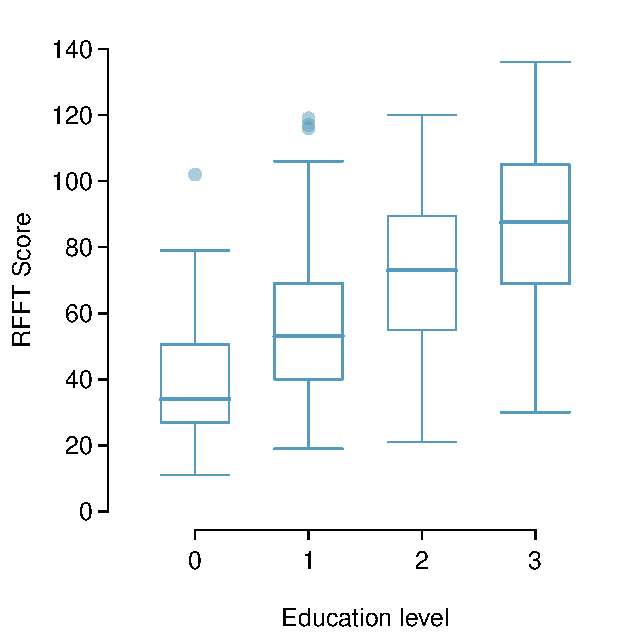
\includegraphics[width=0.55\textwidth]
	{ch_multiple_linear_regression_oi_biostat/figures/prevendRFFTEducBoxPlot/prevendRFFTEducBoxPlot.pdf}
	\caption{Box plots for RFFT score by education level in \data{prevend.samp}.}
	\label{prevendRFFTEducBoxPlot}
\end{figure}

\begin{examplewrap}
\begin{nexample}{Is RFFT score associated with educational level? Interpret the coefficients from the following model. Figure~\ref{prevendRFFTEducationRegression} provides the \textsf{R} output for the regression model of RFFT versus educational level in \data{prevend.samp}. The variable \var{Education} has been converted to \var{Education.factor}, which has levels \texttt{Primary}, \texttt{LowerSecond}, \texttt{HigherSecond}, and \texttt{Univ}.}

It is clearest to start with writing the model equation:
\[\widehat{\text{RFFT}} =  40.94 + 14.78(\text{EduLowerSecond}) + 32.13(\text{EduHigherSecond}) + 44.96(\text{EduUniv})\]

Each of the predictor levels can be thought of as binary variables that can take on either \resp{0} or \resp{1}, where only one level at most can be a \resp{1} and the rest must be \resp{0}, with \resp{1} corresponding to the category of interest. For example, the predicted mean RFFT score for individuals in the Lower Secondary group is given by
\[\widehat{\text{RFFT}} =  40.94 + 14.78(1) + 32.13(0) + 44.96(0) = 55.72. \]
The value of the \texttt{LowerSecond} coefficient, 14.78, is the change in predicted mean RFFT score from the reference category \texttt{Primary} to the \texttt{LowerSecond} category. 

Participants with a higher secondary education scored approximately 32.1 points higher on the RFFT than individuals with only a primary school education, and have estimated mean RFFT score $40.94 + 32.13 = 73.07.$ Those with a university education have estimated mean RFFT score $40.94 + 44.96 = 85.90$.  

The intercept value, 40.94, corresponds to the estimated mean RFFT score for individuals who at most completed primary school. From the regression equation, 
\[\widehat{\text{RFFT}} =  40.94 + 14.78(0) + 32.13(0) + 44.96(0) = 40.94. \]

The $p$-values indicate that the change in mean score between participants with only a primary school education and any of the other categories is statistically significant.
\end{nexample}
\end{examplewrap}

% latex table generated in R 3.3.2 by xtable 1.8-2 package
% Fri Jan  5 11:32:59 2018
\begin{figure}[ht]
	\centering
	\begin{tabular}{rrrrr}
		\hline
		& Estimate & Std. Error & t value & Pr($>$$|$t$|$) \\ 
		\hline
		(Intercept) & 40.9412 & 3.2027 & 12.78 & 0.0000 \\ 
		Education.factorLowerSecond & 14.7786 & 3.6864 & 4.01 & 0.0001 \\ 
		Education.factorHigherSecond & 32.1335 & 3.7631 & 8.54 & 0.0000 \\ 
		Education.factorUniv & 44.9639 & 3.6835 & 12.21 & 0.0000 \\ 
		\hline
	\end{tabular}
	\caption{\textsf{R} summary output for the regression model of RFFT versus educational level in \data{prevend.samp}, with \var{Education} converted to a factor called \var{Education.factor} that has levels \texttt{Primary}, \texttt{LowerSecond}, \texttt{HigherSecond}, and \texttt{Univ}.}
		\label{prevendRFFTEducationRegression}
\end{figure}		
		
\index{multiple linear regression!categorical predictors|)}

\begin{examplewrap}
\begin{nexample}{Suppose that the model for predicting RFFT score from educational level is fitted with \var{Education}, using the original numerical coding with \resp{0}, \resp{1}, \resp{2}, and \resp{3}; the \textsf{R} output is shown in Figure~\ref{prevendRFFTEducationNumRegression}. What does this model imply about the change in mean RFFT between groups? Explain why this model is flawed.}
	
According to this model, the change in mean RFFT between groups increases by 15.158 for any one unit change in \var{Education}. For example, the change in means between the groups coded \resp{0} and \resp{1} is necessarily equal to the change in means between the groups coded \resp{2} and \resp{3}, since the predictor changes by 1 in both cases. 

It is unreasonable to assume that the change in mean RFFT score when comparing the primary school group to the lower secondary group will be equal to the difference in means between the higher secondary group and university group. The numerical codes assigned to the groups are simply short-hand labels, and are assigned arbitrarily. As a consequence, this model would not provide consistent results if the numerical codes were altered; for example, if the primary school group and lower secondary group were relabeled such that the predictor changes by 2, the estimated difference in mean RFFT would change. 
\end{nexample}
\end{examplewrap}

\begin{figure}[ht]
	\centering
	\begin{tabular}{rrrrr}
		\hline
		& Estimate & Std. Error & t value & Pr($>$$|$t$|$) \\ 
		\hline
		(Intercept) & 41.148 & 2.104 & 19.55 & 0.0000 \\ 
		Education & 15.158 & 1.023 & 14.81 & 0.0000 \\ 
		\hline
	\end{tabular}
	\caption{\textsf{R} summary output for the simple regression model of RFFT versus educational level in \data{prevend.samp}, where \var{Education} is treated as a numerical variable. Note that it would be incorrect to fit this model; Figure~\ref{prevendRFFTEducationRegression} shows the results from the correct approach.} 
	\label{prevendRFFTEducationNumRegression}
\end{figure}
		
Categorical variables can be included in multiple regression models with other predictors, as is shown in the next section. Section~\ref{ANOVAandRegression} discusses the connection between ANOVA and regression models with only one categorical predictor.



\section{Reanalyzing the PREVEND data}
\label{reanalyzingStatinDataSet}

\index{data!PREVEND|(}

The earlier models fit to examine the association between cognitive ability and statin use showed that considering statin use alone could be misleading. While older participants tended to have lower RFFT scores, they were also more likely to be taking statins. Age was found to be a \term{confounder} in this setting\textemdash is it the only confounder?

Potential confounders are best identified by considering the larger scientific context of the analysis. For the PREVEND data, there are two natural candidates for potential confounders: education level and presence of cardiovascular disease. The use of medication is known to vary by education levels, often because individuals with more education tend to have higher incomes and consequently, better access to health care; higher educational levels are associated with higher RFFT scores, as shown by model~\ref{prevendRFFTEducationRegression}. Individuals with cardiovascular disease are often prescribed statins to lower cholesterol; cardiovascular disease can lead to vascular dementia and cognitive decline.

Figure~\ref{prevendRFFTStatinAgeEducationCVD} contains the result of a regression of RFFT with statin use, adding the possible confounders age, educational level, and presence of cardiovascular disease. The variables \var{Statin}, \var{Education} and \var{CVD} have been converted to factors, and \var{Age} is a continuous predictor.

The coefficient for statin use shows the importance of adjusting for confounders.  In the initial model for RFFT that only included statin use as a predictor, statin use was significantly associated with decreased RFFT scores. After adjusting for age, statins were no longer significantly associated with RFFT scores, but the model suggested that statin use could be associated with \emph{increased} RFFT scores. This final model suggests that, after adjusting for age, education, and the presence of cardiovascular disease, statin use is associated with an increase in RFFT scores of approximately 4.7 points. The $p$-value for the slope coefficient for statin use is 0.056, which suggests moderately strong evidence of an association (significant at $\alpha = 0.10$, but not $\alpha = 0.05$).

% latex table generated in R 3.3.2 by xtable 1.8-2 package
% Fri Jan  5 11:40:26 2018
\begin{figure}[ht]
\centering
\begin{tabular}{rrrrr}
  \hline
 & Estimate & Std. Error & t value & Pr($>$$|$t$|$) \\ 
  \hline
(Intercept) & 99.0351 & 6.3301 & 15.65 & 0.0000 \\ 
  Statin.factorUser & 4.6905 & 2.4480 & 1.92 & 0.0559 \\ 
  Age & -0.9203 & 0.0904 & -10.18 & 0.0000 \\ 
  Education.factorLowerSecond & 10.0883 & 3.3756 & 2.99 & 0.0029 \\ 
  Education.factorHigherSecond & 21.3015 & 3.5777 & 5.95 & 0.0000 \\ 
  Education.factorUniv & 33.1246 & 3.5471 & 9.34 & 0.0000 \\ 
  CVD.factorPresent & -7.5665 & 3.6516 & -2.07 & 0.0388 \\ 
   \hline
\end{tabular}
\caption{\textsf{R} summary output for the multiple regression model of RFFT versus statin use, age, education, and presence of cardiovascular disease in \data{prevend.samp}.} 
\label{prevendRFFTStatinAgeEducationCVD}
\end{figure}

The $R^2$ for the model is 0.4355; a substantial increase from the model with only statin use and age as predictors, which had an $R^2$ of 0.2852. The adjusted $R^2$ for the model is 0.4286, close to the $R^2$ value, which suggests that the additional predictors increase the strength of the model enough to justify the additional complexity.

\textD{\newpage}

Figure~\ref{prevendRFFTStatinAgeEducCVDResidNormPlot} shows a plot of residuals vs predicted RFFT scores from the model in Figure~\ref{prevendRFFTStatinAgeEducationCVD} and a normal probability plot of the residuals. These plots show that the model fits the data reasonably well. The residuals show a slight increase in variability for larger predicted values, and the normal probability plot shows the residuals depart slightly from normality in the extreme tails.  Model assumptions never hold exactly, and the possible violations shown in this figure are not sufficient reasons to discard the model.

\begin{figure}[h]
	\centering
	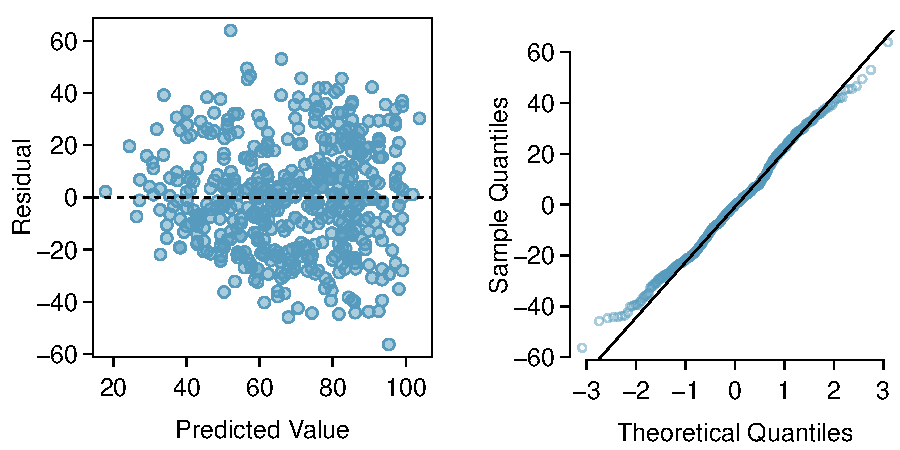
\includegraphics[width=0.8\textwidth]
	{ch_multiple_linear_regression_oi_biostat/figures/prevendRFFTStatinAgeEducCVDResidNormPlot/prevendRFFTStatinAgeEducCVDResidNormPlot.pdf}
	\caption{A histogram and normal probability plot of the residuals from the linear model for RFFT vs. statin use, age, educational level and presence of cardiovascular disease in the PREVEND data.}
	\label{prevendRFFTStatinAgeEducCVDResidNormPlot}
\end{figure}

It is quite possible that even the model summarized in Figure~\ref{prevendRFFTStatinAgeEducationCVD} is not the best one to understand the association of cognitive ability with statin use. There be other confounders that are not accounted for.  Possible predictors that may be confounders but have not been examined are called \term{residual confounders}.  Residual confounders can be other variables in a dataset that have not been examined, or variables that were not measured in the study.  Residual confounders exist in almost all observational studies, and represent one of the main reasons that observational studies should be interpreted with caution. A randomized experiment is the best way to eliminate residual confounders. Randomization ensures that, at least on average, all predictors are not associated with the randomized intervention, which eliminates one of the conditions for confounding.  A randomized trial may be possible in some settings; there have been many randomized trials examining the effect of using statins. However, in many other settings, such as a study of the association of marijuana use and later addiction to controlled substances, randomization may not be possible or ethical.  In those instances, observational studies may be the best available approach.

\index{data!PREVEND|)}


\section{Interaction in regression}
\label{interactionRegression}
\index{multiple linear regression!interaction|(}

An important assumption in the multiple regression model

\[y = \beta_0 + \beta_1x_1 + \beta_2x_2 + ... + \beta_px_p + \varepsilon \] 

is that when one of the predictor variables $x_j$ changes by 1 unit and none of the other variables change, the predicted response changes by $\beta_j$, regardless of the values of the other variables.  A statistical \term{interaction} occurs when this assumption is not true, such that the relationship of one explanatory variable $x_j$ with the response depends on the particular value(s) of one or more other explanatory variables.

Interaction is most easily demonstrated in a model with two predictors, where one of the predictors is categorical and the other is numerical.\footnote{Interaction effects between numerical variables and between more than two variables can be complicated to interpret. A more complete treatment of interaction is best left to a more advanced course; this text will only examine interaction in the setting of models with one categorical variable and one numerical variable.} Consider a model that might be used to predict total cholesterol level from age and diabetes status (either diabetic or non-diabetic):
\begin{align}
E(\text{TotChol}) =& \beta_0 + \beta_1(\text{Age}) + \beta_2(\text{Diabetes}).
\label{nhanesAgeDiabetesModel}
\end{align}

Figure~\ref{nhanesAgeDiabetes} shows the \textsf{R} output for a regression estimating model~\ref{nhanesAgeDiabetesModel}, using data from a sample of 500 adults from the NHANES dataset (\texttt{nhanes.samp.adult.500}). Total cholesterol (\texttt{TotChol}) is measured in mmol/L, \texttt{Age} is recorded in years, and \texttt{Diabetes} is a factor level with the levels \texttt{No} (non-diabetic) and \texttt{Yes} (diabetic) where \texttt{0} corresponds to \texttt{No} and \texttt{1} corresponds to \texttt{Yes}.

% latex table generated in R 3.4.3 by xtable 1.8-2 package
% Sun Mar 11 11:51:34 2018
\begin{figure}[ht]
	\centering
	\begin{tabular}{rrrrr}
		\hline
		& Estimate & Std. Error & t value & Pr($>$$|$t$|$) \\ 
		\hline
		(Intercept) & 4.8000 & 0.1561 & 30.75 & 0.0000 \\ 
		Age & 0.0075 & 0.0030 & 2.47 & 0.0137 \\ 
		DiabetesYes & -0.3177 & 0.1607 & -1.98 & 0.0487 \\ 
		\hline
	\end{tabular}
	\caption{Regression of total cholesterol on age and diabetes, 
		using \texttt{nhanes.samp.adult.500}.} 
	\label{nhanesAgeDiabetes}
\end{figure}

\textD{\newpage}

\begin{examplewrap}
\begin{nexample}{Using the output in Figure~\ref{nhanesAgeDiabetes}, write the model equation and interpret the coefficients for age and diabetes. How does the predicted total cholesterol for a 60-year-old individual compare to that of a 50-year-old individual, if both have diabetes? What if both individuals do not have diabetes?}
	
\[\widehat{TotChol} = 4.80 + 0.0075(Age) - 0.32(DiabetesYes) \]	
The coefficient for age indicates that with each increasing year of age, predicted total cholesterol increases by 0.0075 mmol/L. The coefficient for diabetes indicates that diabetics have an average total cholesterol that is 0.32 mmol/L lower than non-diabetic individuals. 

If both individuals have diabetes, then the change in predicted total cholesterol level can be determined directly from the coefficient for Age. An increase in one year of age is associated with a 0.0075 increase in total cholesterol; thus, an increase in ten years of age is associated with $10(0.0075) = 0.075$ mmol/L increase in predicted total cholesterol.

The calculation does not differ if both individuals are non-diabetic. According to the model, the relationship between age and total cholesterol remains the same regardless of the values of the other variable in the model. 
\end{nexample}
\end{examplewrap}

\begin{examplewrap}
\begin{nexample}{Using the output in Figure~\ref{nhanesAgeDiabetes}, write two separate model equations: one for diabetic individuals and one for non-diabetic individuals. Compare the two models.}\label{nhanesNoInteractionModelFit}%
For non-diabetics (\texttt{Diabetes = 0}), the linear relationship between average cholesterol and age is $\widehat{\text{TotChol}} = 4.80 + 0.0075(\text{Age}) - 0.32(0) = 4.80 + 0.0075(\text{Age}).$

For diabetics (\texttt{Diabetes = 1}), the linear relationship between average cholesterol and age is $\widehat{\text{TotChol}} = 4.80 + 0.0075(\text{Age}) - 0.32(1) = 4.48 + 0.0075(\text{Age}).$

The lines predicting average cholesterol as a function of age in diabetics and non-diabetics are parallel, with the same slope and different intercepts. While predicted total cholesterol is higher overall in non-diabetics (as indicated by the higher intercept), the rate of change in predicted average total cholesterol by age is the same for both diabetics and non-diabetics.

This relationship can be expressed directly from the model equation \ref{nhanesAgeDiabetesModel}. For non-diabetics, the population regression line is $E(\text{TotChol}) = \beta_0 + \beta_1(\text{Age})$. For diabetics, the line is $E(\text{TotChol}) = \beta_0 + \beta_1(\text{Age}) + \beta_2 = \beta_0 + \beta_2 + \beta_1(\text{Age})$. The lines have the same slope $\beta_1$ but intercepts $\beta_0$ and $\beta_0 + \beta_2$.
\end{nexample}
\end{examplewrap}

\textD{\newpage}

However, a model that assumes the relationship between cholesterol and age does not depend on diabetes status might be overly simple and potentially misleading. Figure~\ref{nhanesInteractionScatterPlot} shows a scatterplot of total cholesterol versus age where the least squares models have been fit separately for non-diabetic and diabetic individuals. The blue line in the plot is estimated using only non-diabetic individuals, while the red line was fit using data from diabetic individuals. The lines are not parallel, and in fact, have slopes with different signs. The plot suggests that among non-diabetics, age is positively associated with total cholesterol. Among diabetics, however, age is negatively associated with total cholesterol.

\begin{figure}[h]
	\centering
\subfigure[]{
	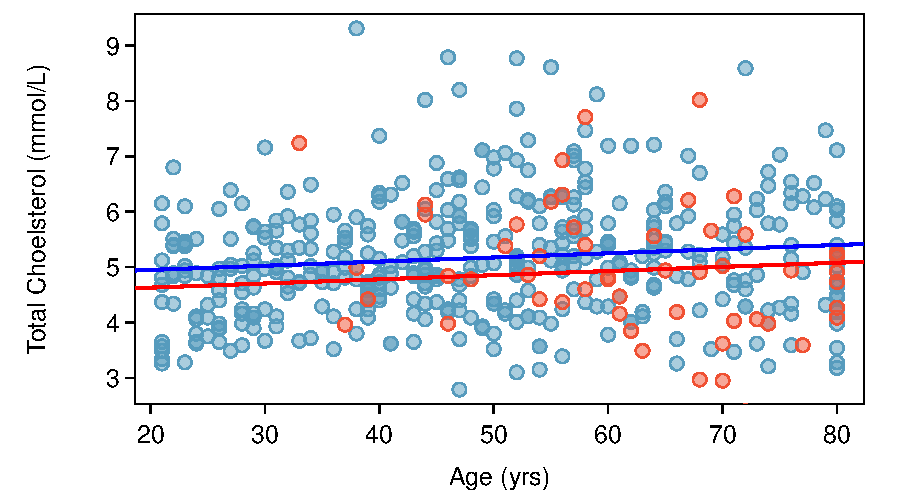
\includegraphics[width=0.65\textwidth]
	{ch_multiple_linear_regression_oi_biostat/figures/nhanesInteractionScatterPlot/nhanesNoInteractionScatterPlot.pdf}
	\label{nhanesNoInteractionScatterPlot}
	}
	\subfigure[]{
		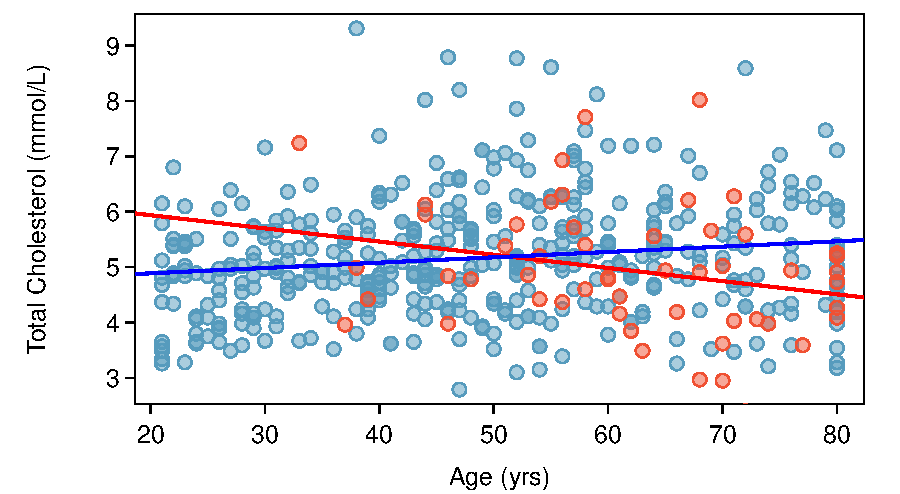
\includegraphics[width=0.65\textwidth]
		{ch_multiple_linear_regression_oi_biostat/figures/nhanesInteractionScatterPlot/nhanesInteractionScatterPlot.pdf}
		\label{nhanesInteractionScatterPlot}
	}
	\caption{Scatterplots of total cholesterol versus age in \texttt{nhanes.samp.adult.500}, where blue represents non-diabetics and red represents diabetics. Plot \subref{nhanesNoInteractionScatterPlot} shows the model equations written out in Example~\ref{nhanesNoInteractionModelFit}, estimated from the entire sample of 500 individuals. Plot \subref{nhanesInteractionScatterPlot} shows least squares models that are fit separately; coefficients of the blue line are estimated using only data from non-diabetics, while those of the red line are estimated using only data from diabetics. }
	\label{nhanesInteractionScatterPlotComparison}
\end{figure}

\textD{\newpage}

With the addition of another parameter (commonly referred to as an interaction term), a linear regression model can be extended to allow the relationship of one explanatory variable with the response to vary based on the values of other variables in the model. Consider the model
\begin{align}\label{nhanesAgeDiabetesInteractionModel}
E(\text{TotChol}) = \beta_0 + \beta_1(\text{Age}) + \beta_2(\text{Diabetes}) + 
\beta_3 (\text{Diabetes} \times \text{Age}). 
\end{align}

The interaction term allows the slope of the association with age to differ by diabetes status. Among non-diabetics (\var{Diabetes} = 0), the model reduces to the earlier one,
\[E(\text{TotChol}) = \beta_0 + \beta_1(\text{Age}). \]

Among the diabetic participants, the model becomes
\begin{align*}
  E(\text{TotChol}) &= \beta_0  + \beta_1(\text{Age}) + \beta_2 + 
       \beta_3 (\text{Age}) \\
       & = \beta_0 + \beta_2 + (\beta_1 + \beta_3)(\text{Age}).
\end{align*}

Unlike in the original model, the slopes of the population regression lines for non-diabetics and diabetics are now different: $\beta_1$ versus $\beta_1 + \beta_3$.

Figure~\ref{nhanesAgeDiabetesInteraction} shows the \textsf{R} output for a regression estimating model~\ref{nhanesAgeDiabetesInteractionModel}. In \textsf{R}, the syntax \texttt{Age:DiabetesYes} represents the (Age $\times$ Diabetes) interaction term. 

% latex table generated in R 3.3.2 by xtable 1.8-2 package
% Fri Jan 12 11:05:33 2018
\begin{figure}[ht]
\centering
\begin{tabular}{rrrrr}
  \hline
 & Estimate & Std. Error & t value & Pr($>$$|$t$|$) \\ 
  \hline
(Intercept) & 4.6957 & 0.1597 & 29.40 & 0.0000 \\ 
  Age & 0.0096 & 0.0031 & 3.10 & 0.0020 \\ 
  DiabetesYes & 1.7187 & 0.7639 & 2.25 & 0.0249 \\ 
  Age:DiabetesYes & -0.0335 & 0.0123 & -2.73 & 0.0067 \\ 
   \hline
\end{tabular}
\caption{Regression of total cholesterol on age and diabetes with an interaction term, using \texttt{nhanes.samp.adult.500}} 
\label{nhanesAgeDiabetesInteraction}
\end{figure}

\begin{examplewrap}
\begin{nexample}{Using the output in Figure~\ref{nhanesAgeDiabetesInteraction}, write the overall model equation, the model equation for non-diabetics, and the model equation for diabetics.}
	
	The overall model equation is 
	\[\widehat{\text{TotChol}} = 4.70 + 0.0096(\text{Age}) + 1.72(\text{DiabetesYes})
	- 0.034(\text{Age} \times \text{DiabetesYes}). \]
	
	For non-diabetics (\texttt{Diabetes = 0}), the linear relationship between average cholesterol and age is
	\[\widehat{\text{TotChol}} = 4.70 + 0.0096(\text{Age}) + 1.72(0)
	- 0.034(\text{Age} \times 0) = 4.70 + 0.0096(\text{Age}).\]
	
	For diabetics (\texttt{Diabetes = 1}), the linear relationship between average cholesterol and age is
	\[\widehat{\text{TotChol}} = 4.70 + 0.0096(\text{Age}) + 1.72(1)
	- 0.034(\text{Age} \times 1) = 6.42 - 0.024(\text{Age}). \]
\end{nexample}
\end{examplewrap}

\textD{\newpage}

The estimated equations for non-diabetic and diabetic individuals show the same qualitative behavior seen in Figure~\ref{nhanesInteractionScatterPlot}, where the slope is positive in non-diabetics and negative in diabetics. However, note that the lines plotted in the figure were estimated from two separate model fits on non-diabetics and diabetics; in contrast, the equations from the interaction model are fit using data from all individuals.

\index{multiple linear regression!interaction|)}

\begin{comment}
JV: Less confusing to hide the following observation, I think. Would require explicitly showing the model coefficients for the lines (which are actually the same in this case) and then a more extended explanation.

However, note that the equations of the lines plotted in the figure are not the same as in the model with the interaction term. 
\end{comment}

It is more efficient to model the data using a single model with an interaction term than working with subsets of the data.\footnote{In more complex settings, such as those with potential interaction between several variables or between two numerical variables, it may not be clear how to subset the data in a way that reveals interactions. This is another advantage to using an interaction term and single model fit to the entire dataset.} Additionally, using a single model allows for the calculation of a $t$-statistic and $p$-value that indicates whether there is statistical evidence of an interaction. The $p$-value for the \texttt{Age:Diabetes} interaction term is significant at the $\alpha = 0.05$ level. Thus, the estimated model suggests there is strong evidence for an interaction between age and diabetes status when predicting total cholesterol. 

Residual plots can be used to assess the quality of the model fit. Figure~\ref{nhanesAgeDiabetesCholResidPlot} shows that the residuals have roughly constant variance in the region with the majority of the data (predicted values between 4.9 and 5.4 mmol/L). However, there are more large positive residuals than large negative residuals, which suggests that the model tends to underpredict; i.e., predict values of \var{TotChol} that are smaller than the observed values.\footnote{Recall that model residuals are calculated as $y_i - \hat{y}_i$; i.e., $\text{TotChol}_i - \widehat{\text{TotChol}}_i$.} Figure~\ref{nhanesAgeDiabetesCholResidNormPlot} shows that the residuals do not fit a normal distribution in the tails. In the right tails, the sample quantiles are larger than the theoretical quantiles, implying that there are too many large residuals. The left tail is a better fit; however, there are too few large negative residuals since the sample quantiles in the left tail are closer to 0 than the theoretical quantiles.

\begin{figure}[h]
	\centering
	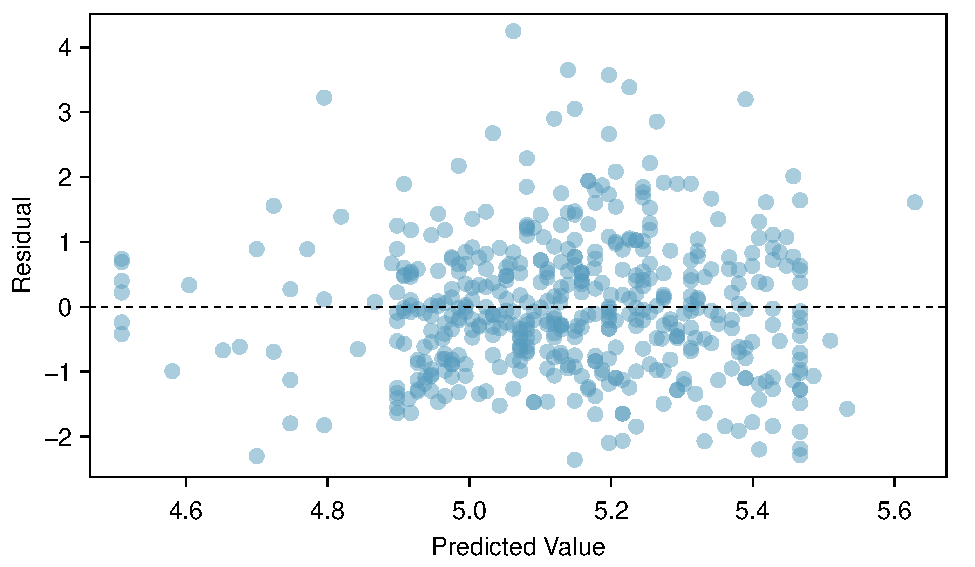
\includegraphics[width=0.8\textwidth]
	{ch_multiple_linear_regression_oi_biostat/figures/nhanesAgeDiabetesCholResidPlot/nhanesAgeDiabetesCholResidPlot.pdf}
	\caption{A scatterplot of residuals versus predicted values in the model for total cholesterol that includes age, diabetes status, and the interaction of age and diabetes status.}
	\label{nhanesAgeDiabetesCholResidPlot}
\end{figure}

\begin{figure}[h]
	\centering
	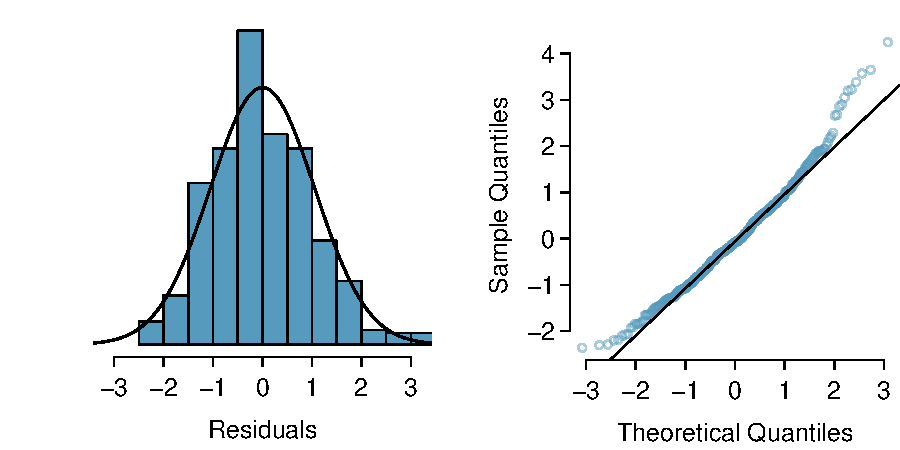
\includegraphics[width=0.8\textwidth]
	{ch_multiple_linear_regression_oi_biostat/figures/nhanesAgeDiabetesCholResidNormPlot/nhanesAgeDiabetesCholResidNormPlot.pdf}
    \caption{A histogram of the residuals and a normal probability plot of the residuals from the linear model for total cholesterol versus age, diabetes status, and the interaction of age and diabetes status.}
   	\label{nhanesAgeDiabetesCholResidNormPlot}
\end{figure}

\textD{\newpage}

It is also important to note that the model explains very little of the observed variability in total cholesterol---the multiple $R^2$ of the model is 0.032. While the model falls well short of perfection, it may be reasonably adequate in applied settings. In the setting of a large study, such as one to examine factors affecting cholesterol levels in adults, a model like the one discussed here is typically a starting point for building a more refined model. Given these results, a research team might proceed by collecting more data. Regression models are commonly used as tools to work towards understanding a phenomenon, and rarely represent a 'final answer'.

There are some important general points that should not be overlooked when interpreting this model. The data cannot be used to infer causality; the data simply show associations between total cholesterol, age, and diabetes status. Each of the NHANES surveys are cross-sectional; they are administered to a sample of US residents with various ages and other demographic features during a relatively short period of time.  No single individual has had his or her cholesterol levels measured over a period of many years, so the model slope for diabetes is not indicative of an individual's cholesterol level declining (or increasing) with age.

Finally, the interpretation of a model often requires additional contextual information that is relevant to the study population but not captured in the dataset. What might explain increased age being associated with lower cholesterol for diabetics, but higher cholesterol for non-diabetics? The guidelines for the use of cholesterol-lowering statins suggest that these drugs should be prescribed more often in older individuals, and even more so in diabetic individuals. It is a reasonable speculation that the interaction between age and diabetes status seen in the NHANES data is a result of more frequent statin use in diabetic individuals.



\section{Model selection for explanatory models}
\label{modelSelection}


\index{multiple linear regression!model selection|(}

Previously, multiple regression modeling was shown in the context of estimating an association while adjusting for possible confounders. Another application of multiple regression is explanatory modeling, in which the goal is to construct a model that explains the observed variation in the response variable. In this context, there is no pre-specified primary predictor of interest; explanatory modeling is concerned with identifying predictors associated with the response. It is typically desirable to have a small model that avoids including variables which do not contribute much towards the $R^2$.

The intended use of a regression model influences the way in which a model is selected. Approaches to model selection vary from those based on careful study of a relatively small set of predictors to purely algorithmic methods that screen a large set of predictors and choose a final model by optimizing a numerical criterion. Algorithmic selection methods have gained popularity as researchers have been able to collect larger datasets, but the choice of an algorithm and the optimization criterion require more advanced material and are not covered here. This section illustrates model selection in the context of a small set of potential predictors using only the tools and ideas that have been discussed earlier in this chapter and in Chapter~\ref{linRegrForTwoVar}. 

Generally, model selection for explanatory modeling follows these steps:

\begin{enumerate}
	\item \textit{Data exploration.} Using numerical and graphical approaches, examine both the distributions of individual variables and the relationships between variables.
	
	\item \textit{Initial model fitting.} Fit an initial model with the predictors that seem most highly associated with the response variable, based on the data exploration.
	
	\item \textit{Model comparison.} Work towards a model that has the highest adjusted $R^2$.
	
	\begin{itemize}
		\item Fit new models without predictors that were either not statistically significant or only marginally so and compare the adjusted $R^2$ between models; drop variables that decrease the adjusted $R^2$. 
		
		\item If the initial set of variables is relatively small, it is prudent to add variables not in the initial model and check the adjusted $R^2$; add variables that increase the adjusted $R^2$.
		
		\item Examine whether interaction terms may improve the adjusted $R^2$.
	\end{itemize}
	
	\item \textit{Model assessment.} Use residual plots to assess the fit of the final model. 
	
\end{enumerate}

The process behind model selection will be illustrated with a case study in which a regression model is built to examine the association between the abundance of forest birds in a habitat patch and features of a patch. 

\index{multiple linear regression!model selection|)}


\textD{\newpage}


\subsubsection{Abundance of forest birds: introduction}

\index{data!forest birds|(}

Habitat fragmentation is the process by which a habitat in a large contiguous space is divided into smaller, isolated pieces; human activities such as agricultural development can result in habitat fragmentation. Smaller patches of habitat are only able to support limited populations of organisms, which reduces genetic diversity and overall population fitness. Ecologists study habitat fragmentation to understand its effect on species abundance. The \data{forest.birds} dataset in the \texttt{oibiostat} package contains a subset of the variables from a 1987 study analyzing the effect of habitat fragmentation on bird abundance in the Latrobe Valley of southeastern Victoria, Australia.\footnote{Loyn, R.H. 1987. "Effects of patch area and habitat on bird abundances, species numbers and tree health in fragmented Victorian forests." Printed in Nature Conservation: The Role of Remnants of Native Vegetation. Saunders DA, Arnold GW, Burbridge AA, and Hopkins AJM eds. Surrey Beatty and Sons, Chipping Norton, NSW, 65-77, 1987.}

The dataset consists of the following variables, measured for each of the 57 patches.
\begin{itemize}
  \item \var{abundance}: average number of forest birds observed in the patch, as calculated from several independent 20-minute counting sessions. 

  \item \var{patch.area}: patch area, measured in hectares. 1 hectare is 10,000 square meters and approximately 2.47 acres.

  \item \var{dist.nearest}: distance to the nearest patch, measured in kilometers.

  \item \var{dist.larger}: distance to the nearest patch larger than the current patch, measured in kilometers.

  \item \var{altitude}: patch altitude, measured in meters above sea level.

  \item \var{grazing.intensity}: extent of livestock grazing, recorded as either "light", "less than average", "average", "moderately heavy", or "heavy". 

  \item \var{year.of.isolation}: year in which the patch became isolated due to habitat fragmentation.

  \item \var{yrs.isolation}: number of years since patch became isolated due to habitat fragmentation.\footnote{The Loyn study completed data collection in 1983;  $\texttt{yrs.isolation} = 1983 - \texttt{year.of.isolation}$.}
\end{itemize}
 
The following analysis is similar to analyses that appear in Logan (2011)\footnote{Logan, M., 2011. Biostatistical design and analysis using R: a practical guide. John Wiley \& Sons, Ch. 9.} and Quinn \& Keough (2002).\footnote{Quinn, G.P. and Keough, M.J., 2002. Experimental design and data analysis for biologists. Cambridge University Press, Ch. 6.} In the approach here, the grazing intensity variable is treated as a categorical variable; Logan and Quinn \& Keough treat grazing intensity as a numerical variable, with values 1-5 corresponding to the categories. The implications of these approaches are discussed at the end of the section.


\textD{\newpage}


\subsubsection{Data exploration}

The response variable for the model is \var{abundance}. Numerical summaries calculated from software show that \var{abundance} ranges from 1.5 to 39.6. Figure~\ref{forestbirdsAbundanceHistandBox} shows that the distribution of \var{abundance} is bimodal, with modes at small values of abundance and at between 25 and 30 birds. The median (21.0) and mean (19.5) are reasonably close, which confirms the distribution is near enough to symmetric to be used in the model without a transformation. The boxplot confirms that the distribution has no outliers.

	\begin{figure}[h]
		\centering
		\subfigure[]{
			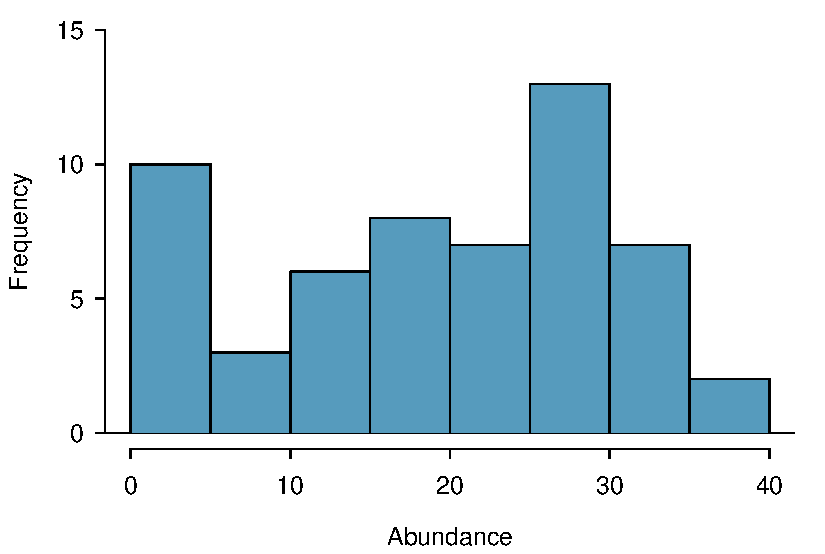
\includegraphics[width=0.55\textwidth]
			{ch_multiple_linear_regression_oi_biostat/figures/forestbirdsAbundanceHist/forestbirdsAbundanceHist}
			\label{forestbirdsAbundanceHist}
		}
    	\subfigure[]{
			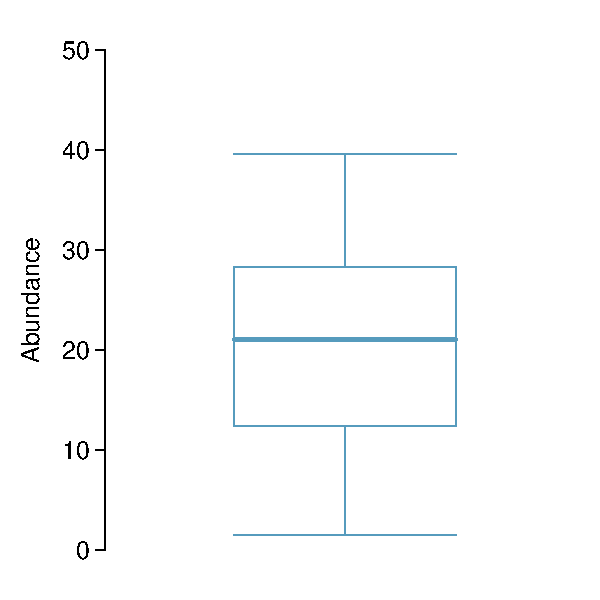
\includegraphics[width=0.38\textwidth]
			{ch_multiple_linear_regression_oi_biostat/figures/forestbirdsAbundanceBox/forestbirdsAbundanceBox}
			\label{forestbirdsAbundanceBox}
		}
		\caption{A histogram \subref{forestbirdsAbundanceHist} and boxplot \subref{forestbirdsAbundanceBox} of \var{abundance} in the \data{forest.birds} data.}
		\label{forestbirdsAbundanceHistandBox}
	\end{figure}	
	
There are six potential predictors in the model; the variable \texttt{year.of.isolation} is only used to calculate the more informative variable \texttt{yrs.isolation}. The plots in Figure~\ref{forestbirdsPredictorDist} reveal right-skewing in \var{patch.area}, \var{dist.nearest}, \var{dist.larger}, and \var{yrs.isolation}; these might benefit from a log transformation. The variable \var{altitude} is reasonably symmetric, and the predictor \var{grazing.factor} is categorical and so does not take transformations. Figure~\ref{forestbirdsLogPredictorDist} shows the distributions of \var{log.patch.area}, \var{log.dist.nearest}, \var{log.dist.larger}, and \var{log.yrs.isolation}, which were created through a natural log transformation of the original variables. All four are more nearly symmetric. These will be more suitable for inclusion in a model than the untransformed versions.

\begin{figure}[h!]
	\centering
	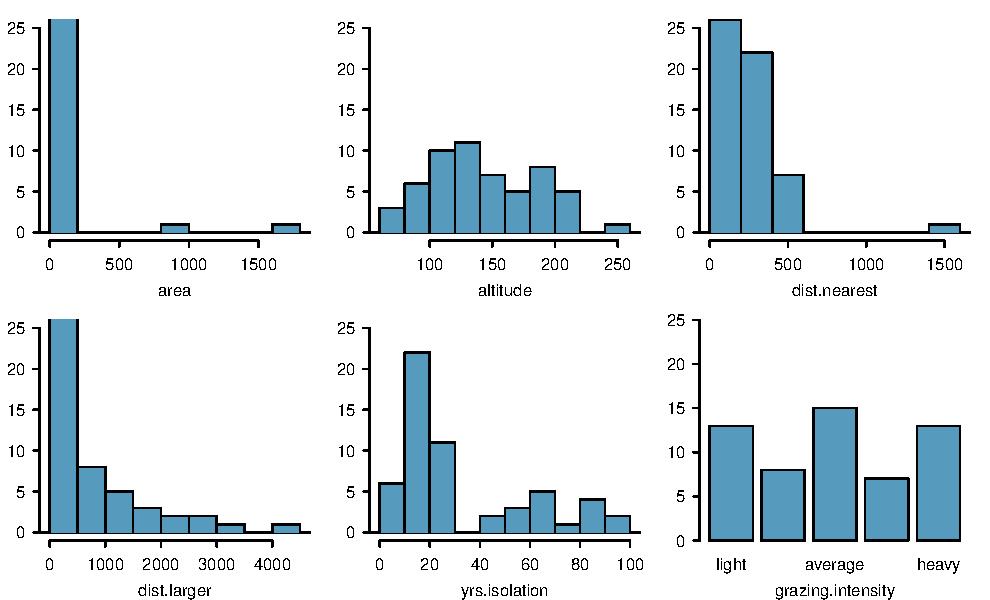
\includegraphics[width=\textwidth]
	{ch_multiple_linear_regression_oi_biostat/figures/forestbirdsPredictorDist/forestbirdsPredictorDist.pdf}
    \caption{Histograms and a barplot for the potential predictors of \var{abundance}.}
   	\label{forestbirdsPredictorDist}
\end{figure}

\textD{\newpage}

\begin{figure}[h!]
	\centering
	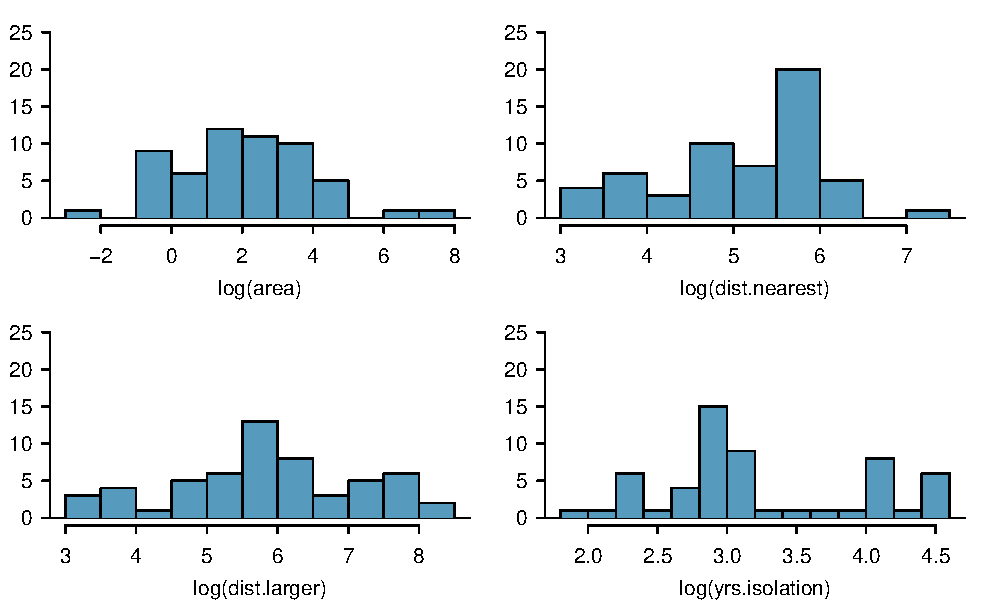
\includegraphics[width=\textwidth]
	{ch_multiple_linear_regression_oi_biostat/figures/forestbirdsLogPredictorDist/forestbirdsLogPredictorDist.pdf}
    \caption{Histograms of the log-transformed versions of \var{patch.area}, \var{dist.nearest}, \var{dist.larger}, and \var{yrs.isolation}.}
   	\label{forestbirdsLogPredictorDist}
\end{figure}

\textD{\newpage}

A \term{scatterplot matrix} can be useful for visualizing the relationships between the predictor and response variables, as well as the relationships between predictors. Each subplot in the matrix is a simple scatterplot; all possible plots are shown, except for the plots of a variable versus itself. The variable names are listed along the diagonal of the matrix, and the diagonal divides the matrix into symmetric plots. For instance, the first plot in the first row shows \var{abundance} on the vertical axis and \var{log.area} on the horizontal axis; the first plot in the first column shows \var{abundance} on the horizontal axis and \var{log.area} on the vertical axis. Note that for readability, \var{grazing.intensity} appears with values 1 - 5, with 1 denoting "light" and 5 denoting "heavy" grazing intensity.

The plots in the first row of Figure~\ref{forestbirdsScatterPlotMatrix} show the relationships between \var{abundance} and the predictors.\footnote{Traditionally, the response variable (i.e., the dependent variable) is plotted on the vertical axis; as a result, it seems more natural to look at the first row where \var{abundance} is on the $y$-axis. It is equally valid, however, to assess the association of \var{abundance} with the predictors from the plots in the first column.} There is a strong positive association between \var{abundance} with \var{log.area}, and a strong negative association between \var{abundance} and \var{log.yrs.isolation}. The variables \var{log.dist.near.patch} and \var{log.dist.larger} seem weakly positively associated with \var{abundance}. There is high variance of \var{abundance} and somewhat similar centers for the first four categories, but \var{abundance} does clearly tend to be lower in the "high grazing" category versus the others.

\begin{figure}[h]
 	\centering
 	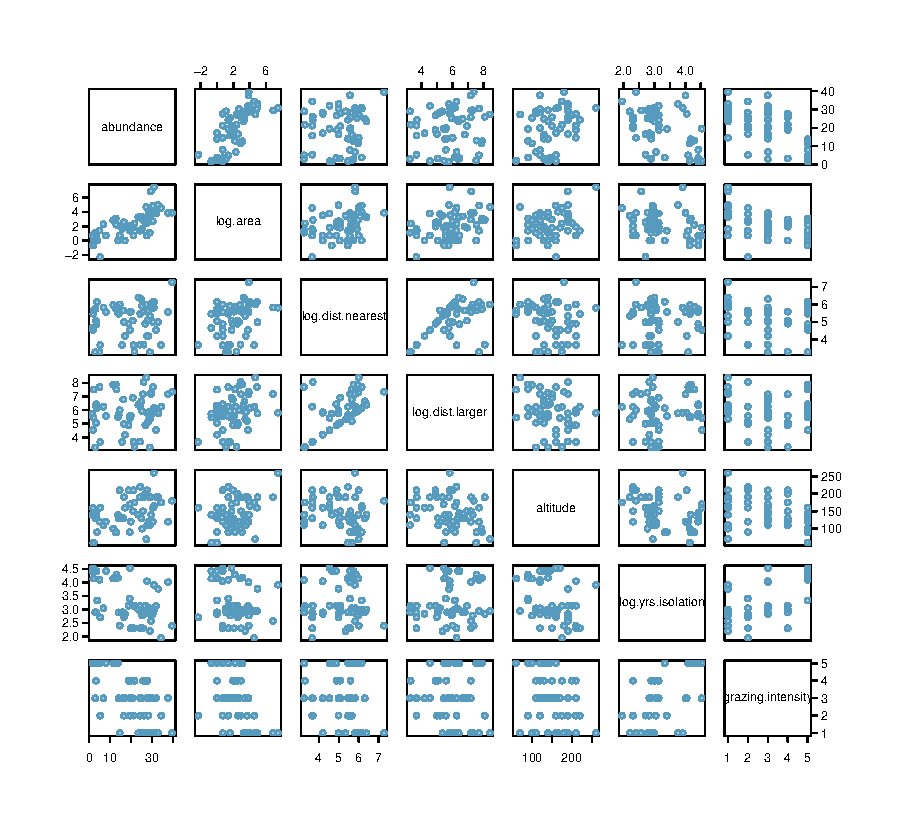
\includegraphics[width=\textwidth]
{ch_multiple_linear_regression_oi_biostat/figures/forestbirdsScatterPlotMatrix/forestbirdsScatterPlotMatrix.pdf}
     \caption{Scatterplot matrix of \var{abundance} and the possible predictors:  \var{log.area}, \var{log.dist.near.patch}, \var{log.dist.larger.patch}, \var{altitude}, \var{log.yrs.isolation}, and \var{grazing.intensity}.}
    	\label{forestbirdsScatterPlotMatrix}
\end{figure} 

\textD{\newpage}

The variables \var{log.dist.nearest} and \var{log.dist.larger} appear strongly associated; a model may only need one of the two, as they may be essentially "redundant" in explaining the variability in the response variable.\footnote{Typically, the predictor that is less strongly correlated with the response variable is the one that is "redundant" and will be statistically insignificant when included in a model with the more strongly correlated predictor. This is not always the case, and depends on the other variables in the model.} In this case, however, since both are only weakly associated with \var{abundance}, both may be unnecessary in a model.

%JV: clearer way to express this other than redundancy?
    
A numerical approach confirms some of the features observable from the scatterplot matrix. Figure~\ref{forestbirdsCorrelation} shows the correlations between pairs of numerical variables in the dataset. Correlations between \var{abundance} and \var{log.area} and between \var{abundance} and \var{log.yrs.isolation} are relatively high, at 0.74 and -0.48, respectively. In contrast, the correlation between \var{abundance} and the two variables \var{log.dist.nearest} and \var{log.dist.larger} are much smaller, at 0.13 and 0.12. Additionally, the two potential predictors \var{log.dist.nearest} and \var{log.dist.larger} have a relatively high correlation of 0.60.

% latex table generated in R 3.4.3 by xtable 1.8-2 package
% Mon Mar 12 23:55:22 2018
\begin{figure}[ht]
	\footnotesize
	\centering
	\begin{tabular}{rrrrrrr}
		\hline
		& abundance & log.area & log.dist.nearest & log.dist.larger & altitude & log.yrs.isolation \\ 
		\hline
		abundance & 1.00 & 0.74 & 0.13 & 0.12 & 0.39 & -0.48 \\ 
		log.area & 0.74 & 1.00 & 0.30 & 0.38 & 0.28 & -0.25 \\ 
		log.dist.nearest & 0.13 & 0.30 & 1.00 & 0.60 & -0.22 & 0.02 \\ 
		log.dist.larger & 0.12 & 0.38 & 0.60 & 1.00 & -0.27 & 0.15 \\ 
		altitude & 0.39 & 0.28 & -0.22 & -0.27 & 1.00 & -0.29 \\ 
		log.yrs.isolation & -0.48 & -0.25 & 0.02 & 0.15 & -0.29 & 1.00 \\ 
		\hline
	\end{tabular}
\caption{A correlation matrix for the numerical variables in \data{forest.birds}.}
\label{forestbirdsCorrelation}
\end{figure}


\subsubsection{Initial model fitting}

Based on the data exploration, the initial model should include the variables \var{log.area}, \var{altitude}, \var{log.yrs.isolation}, and \var{grazing.intensity}; a summary of this model is shown in Figure~\ref{forestbirdsAbunLogAreaAltLogIsolGrazingIntensityRegress}. The $R^2$ and adjusted $R^2$ for this model are, respectively, 0.728 and 0.688.  The model explains about 73\% of the variability in \var{abundance}.  

% latex table generated in R 3.4.3 by xtable 1.8-2 package
% Fri Feb 23 12:36:18 2018
\begin{figure}[ht]
\centering
\begin{tabular}{rrrrr}
  \hline
 & Estimate & Std. Error & t value & Pr($>$$|$t$|$) \\ 
  \hline
(Intercept) & 14.1509 & 6.3006 & 2.25 & 0.0293 \\ 
  log.area & 3.1222 & 0.5648 & 5.53 & 0.0000 \\ 
  altitude & 0.0080 & 0.0216 & 0.37 & 0.7126 \\ 
  log.yrs.isolation & 0.1300 & 1.9193 & 0.07 & 0.9463 \\ 
  grazing.intensityless than average & 0.2967 & 2.9921 & 0.10 & 0.9214 \\ 
  grazing.intensityaverage & -0.1617 & 2.7535 & -0.06 & 0.9534 \\ 
  grazing.intensitymoderately heavy & -1.5936 & 3.0350 & -0.53 & 0.6019 \\ 
  grazing.intensityheavy & -11.7435 & 4.3370 & -2.71 & 0.0094 \\ 
   \hline
\end{tabular}
\caption{Initial model: regression of \var{abundance} on \var{log.area}, \var{altitude}, \var{log.yrs.isolation} and \var{grazing.intensity}.}
\label{forestbirdsAbunLogAreaAltLogIsolGrazingIntensityRegress}
\end{figure}

Two of the variables in the model are not statistically significant at the $\alpha = 0.05$ level: \var{altitude} and \var{log.yrs.isolation}. Only one of the categories of \var{grazing.intensity} (heavy grazing) is highly significant.


\textD{\newpage}


\subsubsection{Model comparison}

First, fit models excluding the predictors that were not statistically significant: \var{altitude} and \var{log.yrs.isolation}. Models excluding either variable have adjusted $R^2$ of 0.69, and a model excluding both variables has an adjusted $R^2$ of 0.70, a small but noticeable increase from the initial model. This suggests that these two variables can be dropped. At this point, the working model includes only \var{log.area} and \var{grazing.intensity}; this model has $R^2 = 0.727$ and is shown in Figure~\ref{forestbirdsAbunLogAreaGrazingRegress}. 

% latex table generated in R 3.4.3 by xtable 1.8-2 package
% Tue Mar 13 21:43:36 2018
\begin{figure}[h]
	\centering
	\begin{tabular}{rrrrr}
		\hline
		& Estimate & Std. Error & t value & Pr($>$$|$t$|$) \\ 
		\hline
		(Intercept) & 15.7164 & 2.7674 & 5.68 & 0.0000 \\ 
		log.area & 3.1474 & 0.5451 & 5.77 & 0.0000 \\ 
		grazing.intensityless than average & 0.3826 & 2.9123 & 0.13 & 0.8960 \\ 
		grazing.intensityaverage & -0.1893 & 2.5498 & -0.07 & 0.9411 \\ 
		grazing.intensitymoderately heavy & -1.5916 & 2.9762 & -0.53 & 0.5952 \\ 
		grazing.intensityheavy & -11.8938 & 2.9311 & -4.06 & 0.0002 \\ 
		\hline
	\end{tabular}
	\caption{Working model: regression of \var{abundance} on \var{log.area} and \var{grazing.intensity}.}
	\label{forestbirdsAbunLogAreaGrazingRegress}
\end{figure}

It is prudent to check whether the two distance-related variables that were initially excluded might increase the adjusted $R^2$, even though this seems unlikely. When either or both of these variables are added, the adjusted $R^2$ decreases from 0.70 to 0.69. Thus, these variables are not added to the working model. 

In this working model, only one of the coefficients associated with grazing intensity is statistically significant; when compared to the baseline grazing category (light grazing), heavy grazing is associated with a reduced predicted mean abundance of 11.9 birds (assuming that \var{log.area} is held constant). Individual categories of a categorical variable cannot be dropped, so a data analyst has the choice of leaving the variable as is, or collapsing the variable into fewer categories. For this model, it might be useful to collapse grazing intensity into a two-level variable, with one category corresponding to the original classification of heavy, and another category corresponding to the other four categories; i.e., creating a version of grazing intensity that only has the levels "heavy" and "not heavy". This is supported by the data exploration; a plot of \var{abundance} versus \var{grazing.intensity} shows that the centers of the distributions of \var{abundance} in the lowest four grazing intensity categories are roughly similar, relative to the center in the heavy grazing category. The model with the binary version of grazing intensity, \var{grazing.binary}, is shown in Figure~\ref{forestbirdsAbunLogAreaGrazingLevelRegress}. The model with \var{grazing.binary} has adjusted $R^2 = 0.71$, which is slightly larger than 0.70 in the more complex model with \var{grazing.intensity}; the model explains 72\% of the variability in \var{abundance} ($R^2 = 0.724$). 

Incorporating an interaction term did not improve the model; adding a parameter for the interaction between \var{log.area} and \var{grazing.binary} decreased the adjusted $R^2$ to 0.709. Thus, the model shown in Figure~\ref{forestbirdsAbunLogAreaGrazingLevelRegress} is the final model.

% latex table generated in R 3.4.3 by xtable 1.8-2 package
% Tue Mar 13 22:26:55 2018
\begin{figure}[ht]
	\centering
	\begin{tabular}{rrrrr}
		\hline
		& Estimate & Std. Error & t value & Pr($>$$|$t$|$) \\ 
		\hline
		(Intercept) & 15.3736 & 1.4507 & 10.60 & 0.0000 \\ 
		log.area & 3.1822 & 0.4523 & 7.04 & 0.0000 \\ 
		grazing.binaryheavy & -11.5783 & 1.9862 & -5.83 & 0.0000 \\ 
		\hline
	\end{tabular}
	\caption{Final model: regression of \var{abundance} on \var{log.area} and \var{grazing.binary}.}
	\label{forestbirdsAbunLogAreaGrazingLevelRegress}
\end{figure}


\textD{\newpage}


\subsubsection{Model assessment}

The fit of a model can be assessed using various residual plots. Figure~\ref{forestbirdsAbunLogAreaGrazingNormPlots} shows a histogram and normal probability plot of the residuals for the final model. Both show that the residuals follow the shape of a normal density in the middle range (between -10 and 10) but fit less well in the tails. There are too many large positive and large negative values) residuals.

 \begin{figure}[h]
 	\centering
 	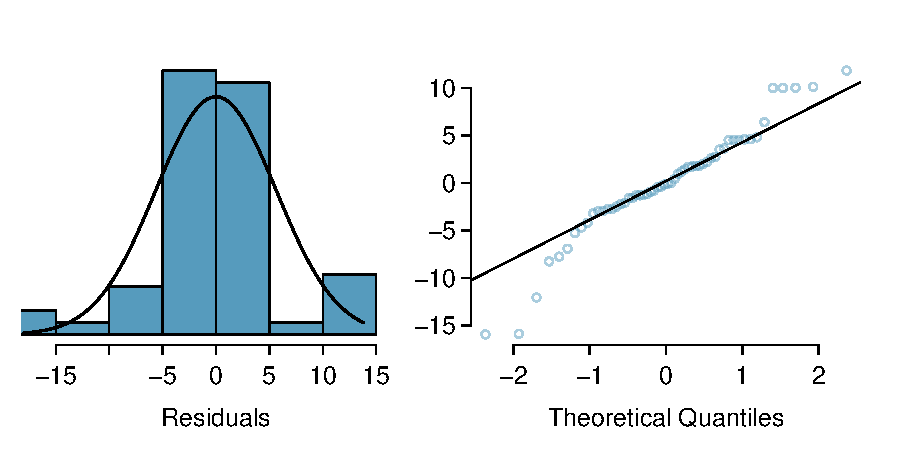
\includegraphics[width=0.8\textwidth]
{ch_multiple_linear_regression_oi_biostat/figures/forestbirdsAbunLogAreaGrazingNormPlots/forestbirdsAbunLogAreaGrazingNormPlots.pdf}
     \caption{Histogram and normal probability plot of residuals in the model for \var{abundance} with predictors \var{log.area} and \var{grazing.binary}.}
    	\label{forestbirdsAbunLogAreaGrazingNormPlots}
 \end{figure}

Figure~\ref{forestbirdsAbunLogAreaGrazingResidPlots} gives a more detailed look at the residuals, plotting the residuals against predicted values and against the two predictors in the model, \var{log.area} and \var{grazing.level}. Recall that residual values closer to 0 are indicative of a more accurate prediction; positive values occur when the predicted value from the model is smaller than the observed value, and vice versa for negative values. Residuals are a measure of the prediction error of a model.

\begin{figure}[h]
	\centering
	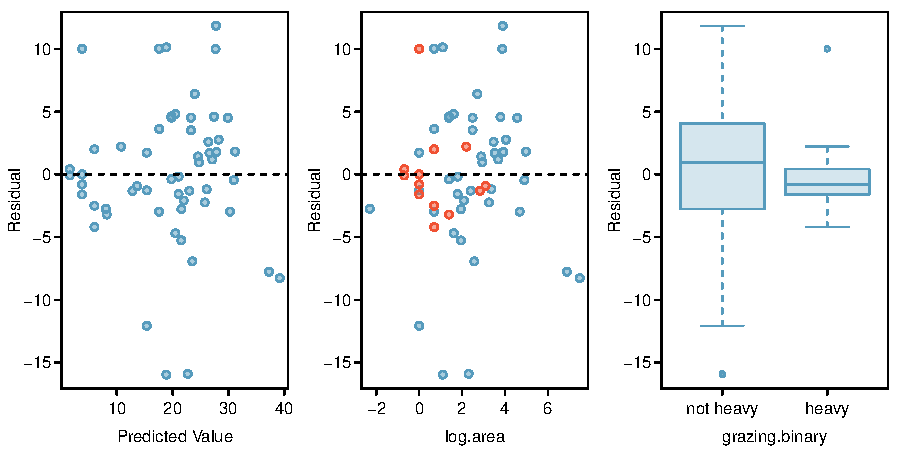
\includegraphics[width=\textwidth]
	{ch_multiple_linear_regression_oi_biostat/figures/forestbirdsAbunLogAreaGrazingResidPlots/forestbirdsAbunLogAreaGrazingResidPlots.pdf}
	\caption{Scatterplots of residuals versus predicted values and residuals versus \var{log.area}, and a side-by-side boxplot of residuals by \var{grazing.binary}. In the middle plot, red points correspond to values where grazing level is "heavy" and blue points correspond to "not heavy".}
	\label{forestbirdsAbunLogAreaGrazingResidPlots}
\end{figure}

\textD{\newpage}

In the left plot, the large positive and large negative residuals visible from Figure~\ref{forestbirdsAbunLogAreaGrazingNormPlots} are evident; the large positive residuals occur across the range of predicted values, while the large negative residuals occur around 20 (predicted birds). The middle plot shows that the large positive and negative residuals occur at intermediate values of \var{log.area}; i.e., for values of \var{log.area} between 0 and 4, or equivalently for values of area between $\exp(0) = 1$ and $\exp(4) = 54.5$ hectares. In the same range, there are also relatively accurate predictions; most residuals are between -5 and 5. Both the middle plot and the right plot show that the prediction error is smaller for patches with heavy grazing than for patches where grazing intensity was between "light" and "moderately heavy". Patches with heavy grazing are represented with red points; note how the red points mostly cluster around the $y = 0$ line, with the exception of one outlier with a residual value of about 10.

\subsubsection{Conclusions}

The relatively large $R^2$ for the final model (0.72) suggests that patch area and extent of grazing (either heavy or not) explain a large amount of the observed variability in bird abundance. Of the features measured in the study, these two are the most highly associated with bird abundance. Larger area is associated with an increase in abundance; when grazing intensity does not change, the model predicts an increase in average abundance by 3.18 birds for every one unit increase in log area (or equivalently, for every $\exp(1) 2.7$ hectares increase in area). A patch with heavy grazing is estimated to have a mean abundance of about 11.58 birds lower than a patch that has not been heavily grazed. 

The residual plots imply that the final model may not be particularly accurate. For most observations, the predictions are accurate between $\pm 5$ birds, but there are several instances of over-predictions as high as around 10 and under-predictions of about 15. Additionally, the accurate and inaccurate predictions occur at similar ranges of of \var{log.area}; if the model only tended to be inaccurate at a specific range, such as for patches with low area, it would be possible to provide clearer advice about when the model is unreliable. The residuals plots do suggest that the model is more reliable for patches with heavy grazing, although there is a slight tendency towards over-prediction.

Based on these results, the ecologists might decide to proceed by collecting more data. Currently, the model seems to adequately explain the variability in bird abundance for patches that have been heavily grazed, but perhaps there are additional variables that are associated with bird abundance, especially in patches that are not heavily grazed. Adding these variables might improve model residuals, in addition to raising $R^2$. 


\subsubsection{Final considerations}

Might a model including all the predictor variables be better than the final model with only \var{log.area} and \var{grazing.binary}? The model is shown in Figure~\ref{forestbirdsFullModel}. The $R^2$ for this model is 0.729 and the adjusted $R^2$ is 0.676. While the $R^2$ is essentially the same as for the final model, the adjusted $R^2$ is noticeably lower. The residual plots in Figure~\ref{forestbirdsAbunFullModelResidNormPlots} do not indicate that this model is an especially better fit, although the residuals are slightly closer to normality. There would be little gained from using the larger model.

% latex table generated in R 3.4.3 by xtable 1.8-2 package
% Fri Feb 23 13:38:29 2018
\begin{figure}[ht]
\centering
\begin{tabular}{rrrrr}
  \hline
 & Estimate & Std. Error & t value & Pr($>$$|$t$|$) \\ 
  \hline
(Intercept) & 10.8120 & 9.9985 & 1.08 & 0.2852 \\ 
  log.area & 2.9720 & 0.6587 & 4.51 & 0.0000 \\ 
  log.dist.near.patch & 0.1390 & 1.1937 & 0.12 & 0.9078 \\ 
  log.dist.larger.patch & 0.3496 & 0.9301 & 0.38 & 0.7087 \\ 
  altitude & 0.0117 & 0.0233 & 0.50 & 0.6169 \\ 
  log.yrs.isolation & 0.2155 & 1.9635 & 0.11 & 0.9131 \\ 
  grazing.intensityless than average & 0.5163 & 3.2631 & 0.16 & 0.8750 \\ 
  grazing.intensityaverage & 0.1344 & 2.9870 & 0.04 & 0.9643 \\ 
  grazing.intensitymoderately heavy & -1.2535 & 3.2000 & -0.39 & 0.6971 \\ 
  grazing.intensityheavy & -12.0642 & 4.5657 & -2.64 & 0.0112 \\ 
   \hline
\end{tabular}
\caption{Full model: regression of \var{abundance} on all 6 predictors in \data{forest.birds}.}
\label{forestbirdsFullModel}
\end{figure}

\begin{figure}[h]
 	\centering
 	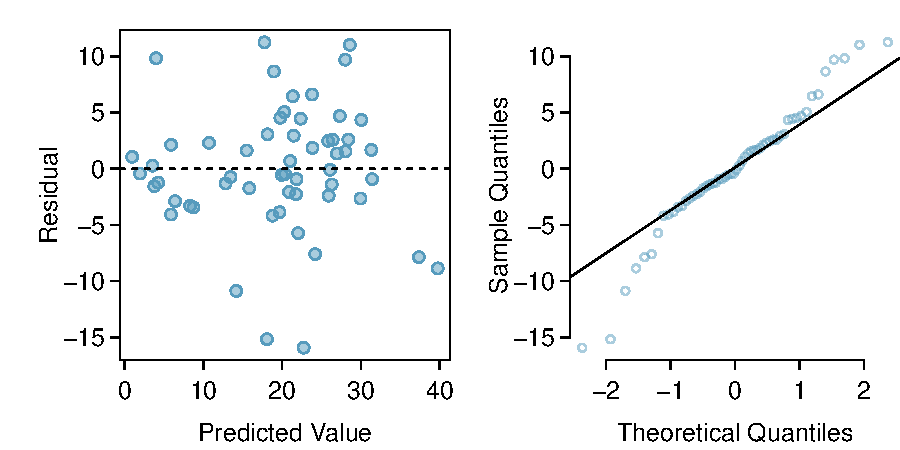
\includegraphics[width=0.8\textwidth]
{ch_multiple_linear_regression_oi_biostat/figures/forestbirdsAbunFullModelResidNormPlots/forestbirdsAbunFullModelResidNormPlots.pdf}
     \caption{Residual plots for the full model of \var{abundance} that includes all predictors.}
    	\label{forestbirdsAbunFullModelResidNormPlots}
 \end{figure}

In fact, there is an additional reason to avoid the larger model. When building regression models, it is important to consider that the complexity of a model is limited by sample size (i.e., the number of observations in the data). Attempting to estimate too many parameters from a small dataset can produce a model with unreliable estimates; the model may be 'overfit', in the sense that it fits the data used to build it particularly well, but will fail to generalize to a new set of data. Methods for exploring these issues are covered in more advanced regression courses. 

\textD{\newpage}

A general rule of thumb is to avoid fitting a model where there are fewer than 10 observations per parameter; e.g., to fit a model with 3 parameters, there should be at least 30 observations in the data. In a regression context, all of the following are considered parameters: an intercept term, a slope term for a numerical predictor, a slope term for each level of a categorical predictor, and an interaction term. In \data{forest.birds}, there are 56 cases, but fitting the full model involves estimating 10 parameters. The rule of thumb suggests that for these data, a model can safely support at most 5 parameters. 

As mentioned earlier, other analyses of \data{forest.birds} have treated \var{grazing.intensity} as a numerical variable with five values. One advantage to doing so is to produce a more stable model; only one slope parameter needs to be estimated, rather than four. However, treating \var{grazing.intensity} as a numerical variable requires assuming that any one unit change is associated with the same change in population mean \var{abundance}; under this assumption, a change between "light" and "less than average" (codes \resp{1} to \resp{2}) is associated with the same change in population mean \var{abundance} as between "moderately heavy" to "heavy" (codes \resp{4} to \resp{5}) grazing. Previous model fitting has shown that this assumption is not supported by the data, and that changes in mean \var{abundance} between adjacent levels in grazing intensity are not constant. In this text, it is our recommendation that categorical variables should not be treated as numerical variables.  

\index{data!forest birds|)}


\section{The connection between ANOVA and regression}
\label{ANOVAandRegression}

\index{multiple linear regression!ANOVA, connection with|(}

Regression with categorical variables and ANOVA are essentially the same method, but with some important differences in the information provided by the analysis. Earlier in this chapter, the strength of the association between RFFT scores and educational level was assessed with regression. Figure~\ref{prevendANOVARFFTEduc} shows the results of an ANOVA to analyze the difference in RFFT scores between education groups.

% latex table generated in R 3.4.3 by xtable 1.8-2 package
% Wed Feb 28 09:44:25 2018
\begin{figure}[ht]
\centering
\begin{tabular}{lrrrrr}
  \hline
 & Df & Sum Sq & Mean Sq & F value & Pr($>$F) \\ 
  \hline
as.factor(Education) & 3 & 115040.88 & 38346.96 & 73.30 & 0.0000 \\ 
  Residuals            & 496 & 259469.32 & 523.12 &  &  \\ 
   \hline
\end{tabular}
\caption{Summary of ANOVA of RFFT by Education Levels} 
\label{prevendANOVARFFTEduc}
\end{figure}

In this setting, the $F$-statistic is used to test the null hypothesis of no difference in mean RFFT score by educational level against the alternative that at least two of the means are different. The $F$-statistic is 73.3 and highly significant. 

The $F$-statistic can also be calculated for regression models, although it has not been shown in the regression model summaries in this chapter. In regression, the $F$-statistic tests the null hypothesis that all regression coefficients are equal to 0 against the alternative that least one of the coefficients is not equal to 0. 

Although the phrasing of the hypotheses in ANOVA versus regression may seem different initially, they are equivalent. Consider the regression model for predicting RFFT from educational level---each of the coefficients in the model is an estimate of the difference in mean RFFT for a particular education level versus the baseline category of $\text{Education} = 0$. A significant $F$-statistic indicates that at least one of the coefficients is not zero; i.e., that at least one of the mean levels of RFFT differs from the baseline category. If all the coefficients were to equal zero, then the differences between the means would be zero, implying all the mean RFFT levels are equal. It is reasonable, then, that the $F$-statistic associated with the \var{RFFT} versus \var{Education} regression model is also 73.3. 

The assumptions behind the two approaches are identical.  Both ANOVA and linear regression assume that the groups are independent, that the observations within each group are independent, that the response variable is approximately normally distributed, and that the standard deviations of the response are the same across the groups.  

The regression approach provides estimates of the mean at the baseline category (the intercept) and the differences of the means between each category and the baseline, along with a $t$-statistic and $p$-value for each comparison. From regression output, it is easy to calculate all the estimated means; to do the same with ANOVA requires calculating summary statistics for each group. Additionally, diagnostic plots to check model assumptions are generally easily accessible in most computing software.  

\textD{\newpage}

Why use ANOVA at all if fitting a linear regression model seems to provide more information?  A case can be be made that the most important first step in analyzing the association between a response and a categorical variable is to compute and examine the $F$-statistic for evidence of any effect, and that only when the $F$-statistic is significant does it become appropriate to proceed to examine the nature of the differences. ANOVA displays the $F$-statistic prominently, emphasizing its importance. It is available in regression output, but may not always be easy to locate; the focus of regression is on the significance of the individual coefficients.  ANOVA has traditionally been used in carefully designed experiments. There are complex versions of ANOVA that are appropriate for experiments in which several different factors are set at a range of levels.  More complex versions of ANOVA are beyond the scope of this text and are covered in more advanced books. 

Section~\ref{anovaAndRegrWithCategoricalVariables} discussed the use of Bonferroni corrections when testing hypotheses about pairwise differences among the group means when conducting ANOVA. In principle, Bonferroni corrections can be applied in regression with categorical variables, but that is not often done. In designed experiments in which ANOVA has historically been used, the goal was typically to show definitively that a categorical predictor, often a treatment or intervention, was associated with a response variable so that the treatment could be adopted for clinical use. In experiments where the predictor can be manipulated by a scientist and cases are randomized to one of several levels of a predictor, the association can be interpreted as causal.  It can be particularly important to control Type I error probabilities in those settings.  Regression is often thought of as an exploratory technique, used in observational studies to discover associations that can be explored in further studies.  Strict control of Type I error probabilities may be less critical in such settings.

At the introductory level, ANOVA is useful in that it provides more direct access to Type I error control and pairwise comparisons with $t$-tests. In practice, with the use of techniques not covered in this text, any analysis done via the ANOVA approach can also be approached with regression modeling. 


\index{multiple linear regression!ANOVA, connection with|)}


\section{Notes}
\label{multLinRegrNotes}

This chapter and the previous chapter cover only the basic principles behind linear regression, and are meant to provide useful tools for getting started with data analysis. This section summarizes the most important ideas in the chapter and makes reference to some related topics that have not been discussed in detail.

\subsubsection{Important ideas}

\begin{description}

	\item \emph{Keep a clear view of the purpose.} Is the goal of constructing the model to understand the relationship between the response and a particular predictor after adjusting for confounders? Or is the goal to understand the joint association between a response and a set of predictors? 
	
	\item \emph{Avoid rushing into model fitting.} Before fitting models, examine the data. Assess whether the response variable has an approximate normal distribution, or at least a symmetric distribution; a log transformation will often produce approximate normality. Examine the relationships between the response and predictors, as well as the relationships between predictors; check for nonlinear trends or outliers. 
	
	\item \emph{Remember the context of the problem.} Context is important at each stage of a regression analysis. The best approach for constructing a model from a small number of potential predictors is based on considering the context of the problem and including predictors that have either been shown in the past to be associated with the response or for which there is a plausible working hypothesis about association with the response. When interpreting coefficients, consider whether the model results cohere with the underlying biological or medical context.
	
	\item \emph{Critically examine residual plots.} All models are approximations, so it is not necessary to be concerned about relatively minor violations of assumptions; residual plots are seldom as well behaved as those for the PREVEND data. In some cases, like with the California DDS data, residual plots show obvious major violations. With intermediate cases such as in the \data{forest.birds} plots, examine the plots closely and provide a detailed assessment of where the model seems less reliable.

\end{description}


\textD{\newpage}


\subsubsection{Related topics}

\begin{description}
	\item \emph{Stepwise model selection.} Many introductory texts recommend using ``stepwise'' regression. Forward stepwise regression adds predictors one by one according to a set criterion (usually by smallest $p$-value). Backward stepwise regression eliminates variables one by one from a larger model until a criterion is met. Stepwise methods can be useful, and are usually automated in statistical software. However, there are weaknesses---the final models are data-dependent and chance alone can lead to spurious variables being included. In very large datasets, stepwise regression can lead to substantially incorrect models.
	
	\item \emph{Prediction models.} An application of regression not discussed in this chapter is predictive modeling, in which the goal is to construct a model that best predicts outcomes. The focus is on overall predictive accuracy; significance of individual coefficients is less important. Evaluating a model's predictive accuracy involves advanced methods such as cross-validation, in which the original data sample is divided into a training set and a test set, similar to the approach used with the Golub leukemia data in Chapter~\ref{introductionToData}. Prediction models are typically built from large datasets, using automated model selection procedures like stepwise regression.
	
	\item \emph{Prediction intervals.} Predicted values from regression have an inherent uncertainty because model parameters are only estimates. There are two types of interval estimates used with prediction: confidence intervals for a predicted mean response from a set of values for the predictors, and prediction intervals that show the variability in the predicted value for a new response (i.e., for a case not in the dataset) given a set of values for the predictor variables. Prediction intervals are wider than confidence intervals for a predicted mean because prediction intervals are subject to both the variability in a predicted mean response and the variability of an individual observation about its mean.
	
	\item \emph{Controlling Type I error in regression.} Control of Type I error probabilities becomes more critical in regression models with very large numbers of potential predictors. Datasets containing measurements on genetic data often contain large numbers of potential predictors for a response for many cases; a stricter significance level is used to maintain an overall error rate of $\alpha = 0.05$. For example, in genome-wide association studies, the accepted "genome-wide significance rate" for an individual marker to be considered significantly associated with an outcome is $5 \times 10^{-8}$.
	
\end{description}

Because there are so many tools available in multiple regression, this chapter has a larger collection of labs than most other chapters. Lab 1 introduces the multiple regression model, illustrating one its most common uses---estimating an association between a response variable and predictor of interest while adjusting for possible confounding. Lab 2 discusses the residual plots used to check assumptions for multiple regression and introduces adjusted $R^2$ using the California DDS dataset initially introduced in Chapter~\ref{introductionToData}. 

Lab 3 explores how the association between a response variable and categorical predictors with more than two levels can be be estimated using multiple regression. This topic extends the earlier material in Chapter 6, Lab 4. Lab 4 introduces the concept of a statistical interaction using the NHANES dataset, examining whether the association between BMI and age among women is different than that among men. 

Multiple regression is often used to examine associations between response variables and a small set of pre-specified predictors. It can also be used to explore and select models between a response variable and a set of candidate predictors. Lab 5 discusses explanatory modeling, in which the goal is to construct a model that effectively explains the observed variation in the response variable. 
